\documentclass[12pt,letter]{article}
\usepackage{../downey_format}


\begin{document}
	
	% set the section number, along with figure and equation numbers
	\setcounter{section}{1}	
	\setcounter{figure}{0}   
	\renewcommand\thefigure{\thesection.\arabic{figure}}
	\setcounter{equation}{0}   
	\renewcommand\theequation{\thesection.\arabic{equation}}
	\section{Free Vibrations}





			
		Vibrations (i.e. the exchange of potential and kinetic energy) require oscillatory motion that may repeat itself regularly or irregularly. A motion that is repeated at time intervals is called periodic motion. If this motion has a single frequency and amplitude it is called simple harmonic motion are represents the most basic form of oscillatory motion as depicted in figure \ref{fig:oscillatorymotion}.  For a 1-DOF system, simple harmonic motion is defined as a periodic motion where the restoring force is directly proportional to the displacement and acts in the direction opposite to that of displacement.	
		

		\begin{figure}[H]
			\centering
			\includegraphics[]{../figures/oscillatory_motion.png}
			\caption{Oscillatory motion for a single degree of freedom system showing (a) periodic motion; and (b) simple harmonic motion.}
			\label{fig:oscillatorymotion}
		\end{figure}

		Given the nature of simple harmonic motion, constant amplitude, and frequency, the wave starting at the origin $O$ can be modeled at a point on the end of a vector with length $A$ rotating at a constant angular velocity $\omega_\text{n}$ where the angle from the origin of the vector is $\phi$, defined as $\phi = \omega t$. Where $\omega$ is the lowercase Greek letter Omega and $\phi$ is the lowercase Coptic letter phi. This is similar to a Greek phi ($\varphi$) and either can be used in this context. The subscript $n$ on $\omega$ denotes that this frequency relates to the natural frequency of the system, the only frequency in simple harmonic motion. A visualization of the harmonic motion obtained from projecting the point on the edge of a vector onto the $\omega_\text{n} t$ space is presented in figure \ref{fig:Harmonic_Motion}. 

		\begin{figure}[H]
			\centering
			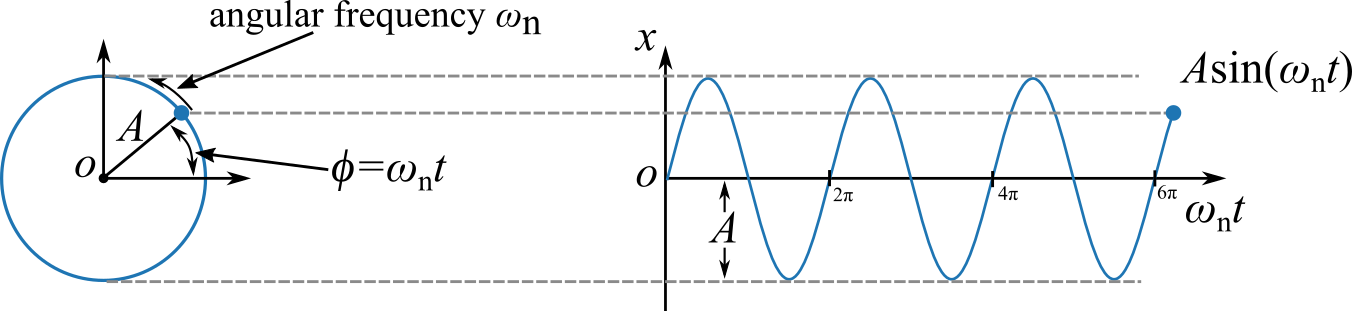
\includegraphics[]{../figures/harmonic_motion.png}
			\caption{Harmonic motion represented at the projection of a point on the end of a vector moving on a circle. Note the axis $\omega_\text{n} t$.}
			\label{fig:Harmonic_Motion}
		\end{figure}

	\subsection{Mathematical Modeling of Free Vibration}

		The Development of a mathematical model for a system under free vibration would enable the practitioner to predict, or model, the vibrating system of interest.  Therefore, considering the following system, 
		
		\begin{figure}[H]
			\centering
			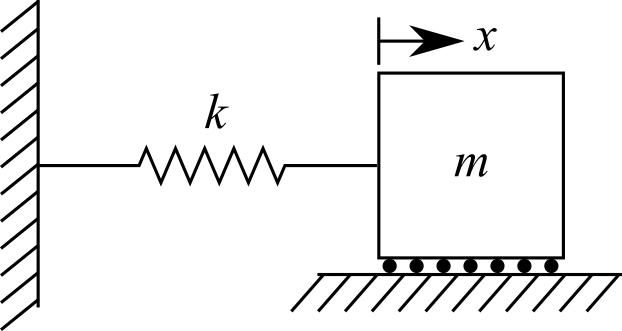
\includegraphics[]{../figures/1-DOF-spring_mass_horizontal.png}
			\caption{1-DOF spring-mass system.}
		\end{figure}
		\noindent can be modeled expressed with the following EOM
		\begin{equation}
			m\ddot{x}(t) + kx(t) = 0
			\label{eq:EOM}
		\end{equation}		
		it becomes prudent to solve this homogeneous ordinary differential equation (ODE) to obtain a model of the vibrating system. 

		The simplest method for solving an ODE is to propose a solution based on observations of a vibrating physical system\protect\footnotemark[1]. Figure \ref{fig:Harmonic_Motion_2.png} reports and annotates the key components from an observation of a vibrating system. 
		
		\footnotetext[1]{Called an ansatz solution. Oxford Languages definition: noun, MATHEMATICS, an assumption about the form of an unknown function which is made in order to facilitate solution of an equation or other problem.} 

		\begin{figure}[H]
			\centering
			\includegraphics[]{../figures/harmonic_motion_2.png}
			\caption{Summary of the temporal response for a 1-DOF system.}
			\label{fig:Harmonic_Motion_2.png}
		\end{figure}
		\noindent where $x_0$ and $v_0$ are the is the displacement and velocity at $t$=0 (i.e. the initial displacement). 
				

		A mathematical expression can now be formulated to represent the observed simple harmonic motion. This expression can be based on the projection of a point on a vector (transposed into the time domain) or assembled from constituent parts as done in what follows. Solving for a location $x$, at a time $t$; $x(t)$, the various characteristics of the expression can be identified:

			\begin{itemize}
				\item System oscillates $\rightarrow$ a sin function models this 
				\item System oscillates at different speed $\rightarrow$ use a parameter to adjust $\omega_\text{n}$ in rad/s. 
				\item Systems have different amplitudes $\rightarrow$ use a parameter to adjust $A$ in meters.
				\item System has different starting points $\rightarrow$ use a parameter to adjust $\phi$ in rad. 
			\end{itemize}

			\noindent Using these four constituent components, an equation can be proposed: 
			\begin{equation}
				{x}(t) = A\text{sin}(\omega_\text{n} t + \phi)
			\end{equation}
			This expression can be shown to be the correct solution of a 1-DOF system through simple experimentation. 

			\subsubsection{Solve for the Natural Frequency ($\omega_\text{n}$) of the System }

			Often, we with to directly compute the natural frequency of a system from its parameters. Take the derivative to get velocity:
			\begin{equation}
				\dot{x}(t) = A\omega_\text{n}\text{cos}(\omega_\text{n} t + \phi)
			\end{equation}
			Take the derivative again to get acceleration:
			\begin{equation}
			\ddot{x}(t) = -A\omega_\text{n}^2\text{sin}(\omega_\text{n} t + \phi)
			\end{equation}
			Substituting $x$ and $\ddot{x}$ into the EOM for the considered 1-DOF system ($m\ddot{x}(t) + kx(t) = 0$) yields:
			\begin{equation}
				m\big(-A\omega_\text{n}^2\text{sin}(\omega_\text{n} t + \phi)\big) + k\big(A\text{sin}(\omega_\text{n} t + \phi)\big) = 0
			\end{equation}
			Thereafter, dividing both sides by $A\text{sin}(\omega_\text{n} t + \phi)$ results in the expression:
			\begin{equation}
				-m\omega_\text{n}^2+k = 0
			\end{equation}
			This expression can be rearranged into the more useful standard form:
			\begin{equation}
				\omega_\text{n}= \sqrt{\frac{k}{m}}
				\label{eq:natural_frequency}
			\end{equation}
			
			Equation \ref{eq:natural_frequency} represents a solution to the EOM  presented in equation \ref{eq:EOM}. This solution is not in the form of an ODE  so, therefore, we can experientially prove that this is the correct solution. For example, we could build a system with known mass and stiffness and measure the natural frequency of the system. Equation \ref{eq:natural_frequency} equation leads to:
			\begin{equation}
				T= \frac{2 \pi}{\omega_\text{n}}
			\end{equation}
			where $T$ is the period of oscillations and 
			\begin{equation}
				f_n= \frac{\omega_\text{n}}{2 \pi}
			\end{equation}
			where $f_n$ is the frequency of the oscillations. 

				\begin{note}
					Radians are considered a dimensionless quantity and as such the units of  $m\omega_\text{n}^2$ become  $\frac{\rm{kg}}{\rm{s}^2}\cdot\frac{\rm{m}}{\rm{m}}$ where the unit value $\frac{\rm{m}}{\rm{m}}$ is added such that the stiffness of the spring can be expressed as $\frac{\rm{kg}\cdot \rm{m}}{\rm{s}^2}\cdot\frac{1}{\rm{m}}$ = $\frac{\rm{N}}{\rm{m}}$.  The International System of Units (SI) defines radians as a derived unit for measuring angles. Interestingly, the topic is still discussed by some  \protect\footnotemark[1]. 
				\end{note}
				\footnotetext[1]{Quincey, Paul. ``Angles in the SI: treating the radian as an independent, unhidden unit does not require the redefinition of the term `frequency' or the unit hertz.'' Metrologia 57.5 (2020):053001.}
					
		\subsubsection{Solve for Initial Phase ($\phi$) of the System }
			The EOM is a second-order ODE so there needs to exist two initial conditions (constants) to solve it. For the systems under consideration, the displacement ($x$) and velocity ($\dot{x}$ or $v$) at $t=0$ are the initial conditions. For simplicity, these are written as 
			\begin{equation}
				x(0) = x_0  
			\end{equation}			
			\begin{equation}
				\dot{x}(0) = v(0) = v_0 
			\end{equation}			
			Setting the equation to its initial state $t=0$, the equations for displacement and velocity can be simplified to: 
			\begin{equation}
				{x}(0) = x_0 = A\text{sin}(\omega_\text{n} 0 + \phi) = A\text{sin}(\phi)
				\label{eq:x_0=Asintheta} 
			\end{equation}
			\begin{equation}
				\dot{x}(0) = v_0 = A\omega_\text{n}\text{cos}(\omega_\text{n}0 + \phi) = A\omega_\text{n}\text{cos}(\phi)
				\label{eq:v_0=Aomegacosphi} 
			\end{equation}
			Thereafter, mathematical meanings for $\phi$ and $A$ can be derived. To do this, $\phi$  can be solved for by rearranging equations \ref{eq:x_0=Asintheta} and \ref{eq:v_0=Aomegacosphi} for $A$:
			\begin{equation}
				A = \frac{x_0}{\text{sin}(\phi) }
			\end{equation}
			and:
			\begin{equation}
				A = \frac{v_0}{\omega_\text{n}\text{cos}(\phi)}
			\end{equation}
			Setting these two equations equal to each other cancels out A and creates:
			\begin{equation}
				\frac{x_0 \omega_\text{n}}{\text{sin}(\phi)} = \frac{v_0}{\text{cos}(\phi)} 
			\end{equation}
			therefore:
			\begin{equation}
				\frac{x_0\omega_\text{n}}{v_0} = \frac{\text{sin}(\phi)}{\text{cos}(\phi)}
			\end{equation}
			finally:
			\begin{equation}
				\phi = \text{tan}^{-1}\bigg(\frac{x_0\omega_\text{n}}{v_0}\bigg)
			\end{equation}
			
		\subsubsection{Solve for Amplitude ($A$) of the System }
			
			The amplitude of the vibrating system ($A$) is solved for in a similar manner to $\phi$ where the expressions for $x$ and $\dot{x}$ are solved for at $t=0$ and rearranged as to isolate $\phi$. This operation results in the equations:  
			\begin{equation}
				\text{sin}(\phi) = \frac{x_0}{A}
			\end{equation}
			and:
			\begin{equation}
				\text{cos}(\phi) = \frac{v_0}{\omega_\text{n}A}
			\end{equation}
			From these equations a value for $\phi$ can be obtained knowing that $\text{sin}(\phi)^2+\text{cos}(\phi)^2=1$. Therefore:
			\begin{equation}
				\bigg(\frac{x_0}{A}\bigg)^2  + \bigg(\frac{v_0}{\omega_\text{n}A}\bigg)^2 = 1
			\end{equation}
			multiplying each expression by 1 (also expressed as $\frac{\omega_\text{n}}{\omega_\text{n}}$), gives the equation:
			\begin{equation}
				\bigg(\frac{\omega_\text{n}}{\omega_\text{n}}\bigg)^2\bigg(\frac{x_0}{A}\bigg)^2  + 1 \bigg(\frac{v_0}{\omega_\text{n}A}\bigg)^2  = 1 \times 1
			\end{equation}
			which becomes:
			\begin{equation}
				\bigg(\frac{\omega_\text{n} x_0}{\omega_\text{n} A}\bigg)^2  + \bigg(\frac{v_0}{\omega_\text{n}A}\bigg)^2 = 1
			\end{equation}
			Further simplification is obtained by multiplying each side by $(\omega_\text{n} A)^2$ to obtain:
			\begin{equation}
				\omega_\text{n}^2x_0^2+v_0^2=A^2\omega_\text{n}^2 
			\end{equation}
			Solving for $A$, this expression rearranges to:
			\begin{equation}
				A = \frac{\sqrt{\omega_\text{n}^2x_0^2+v_0^2}}{\omega_\text{n}} = \sqrt{x_0^2+\bigg(\frac{v_0}{\omega_\text{n}}\bigg)^2}
			\end{equation}
		
		\subsubsection{Response for Simple Harmonic Motion}
			
			The time-varying displacement of a 1-DOF vibrating system under free response is expressed by the equation ${x}(t) = A\text{sin}(\omega_\text{n} t + \phi)$. Substituting in the expressions for $A$ and $\phi$ results in:
			
			\begin{equation}
				{x}(t) = \frac{\sqrt{\omega_\text{n}^2x_0^2+v_0^2}}{\omega_\text{n}}\text{sin}\Bigg(\omega_\text{n} t + \bigg( \text{tan}^{-1}\bigg(\frac{x_0\omega_\text{n}}{v_0}\bigg)\bigg)\Bigg)
				\label{eq:response_simple_harmonic_motion}
			\end{equation}
			
			\noindent This equation provides a mathematical solution that relates displacement of the mass to the initial conditions $x_0$ and $v_0$. The solution is considered a free-response because no input is applied after t=0. The relationship between the initial conditions ($x_0$ and $v_0$) and the amplitude and phase of the response can be expressed using the Pythagorean theorem, $a^2 + b^2 = c^2$, as annotated in figure \ref{fig:Trigonometric_relationship}.
			
			\begin{figure}[H]
				\centering
				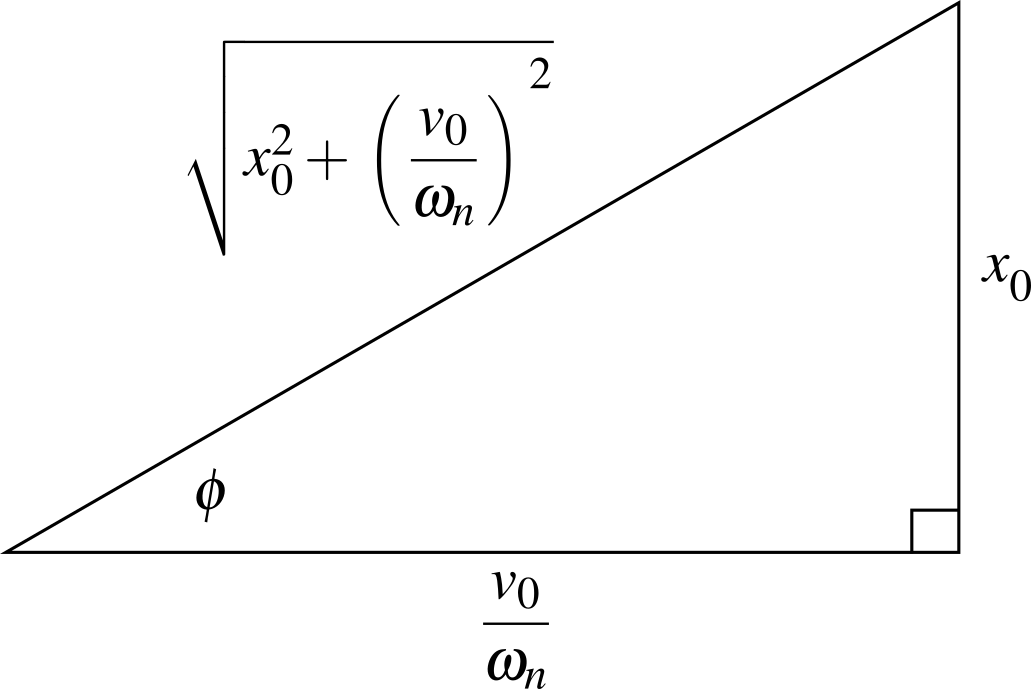
\includegraphics[]{../figures/trigonometric_relationship_undamped_free.png}
				\caption{Trigonometric relationship between the initial conditions ($x_0$ and $v_0$), amplitude $A$, and phase $\phi$ for free vibration of a 1-DOF system.}
				\label{fig:Trigonometric_relationship}
			\end{figure}

		\subsubsection{Special Considerations for No Initial Velocity ($v_0=0$)}
		
			Upon close inspection of the temporal solution in equation \ref{eq:response_simple_harmonic_motion}, it becomes evident that any system without initial velocity (i.e. $v_0=0$) results in an undefined number for $(x_0\omega_\text{n})/v_0$. A solution to this challenge lies in the fact that the limit of tan$^{-1}(x)$ approaches $-\pi/2$ at $-\infty$ and  $\pi/2$ at $\infty$, as depicted in figure \ref{fig:arctan_plot}. Therefore, the solution at $-\infty$ and $\infty$ is undefined, resulting in the expression:
			
			\begin{equation}
				\bigg(\frac{x_0\omega_\text{n}}{v_0}\bigg) = \pm \frac{\pi}{2}, \text{ when } v_0=0
			\end{equation}			
			
			This step is applied in IEEE floating-point arithmetic (IEEE 754) and results in $\pm \pi/2$ depending on the rounding format used. From the practitioner's side, it becomes important to recognize the situation $v_0=0$ and correct this value as needed. 
			
			\begin{figure}[H]
				\centering
				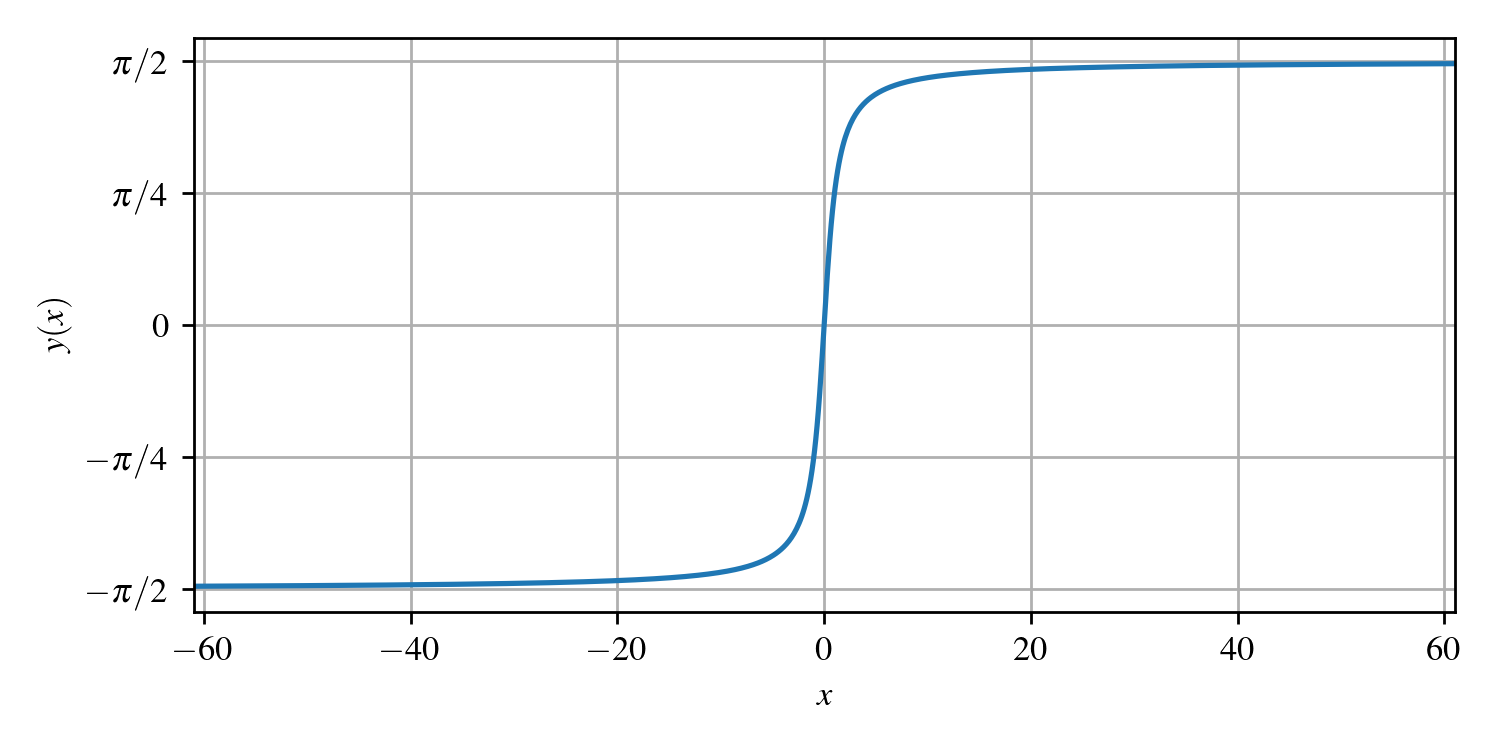
\includegraphics[]{../figures/arctan_plot.png}
				\caption{Response of tan$^{-1}$ (or arctan) for  $x$=-60 to 60 showing that the tan$^{-1}$ is undefined as $x$ approaches $-\infty$ and $\infty$.}
				\label{fig:arctan_plot}
			\end{figure}		
			

			\begin{example}
		
				
			\textbf{Vehicle Suspension Modeling}

			\noindent A vehicle wheel, tire, and suspension can be modeled as an SDOF spring and mass as depicted below: The mass of the wheel and tire is measured to be 300 kg and its frequency of oscillation is observed to be 10 rad/sec. What is the stiffness of the wheel assembly?
				
				\begin{figure}[H]
					\centering
					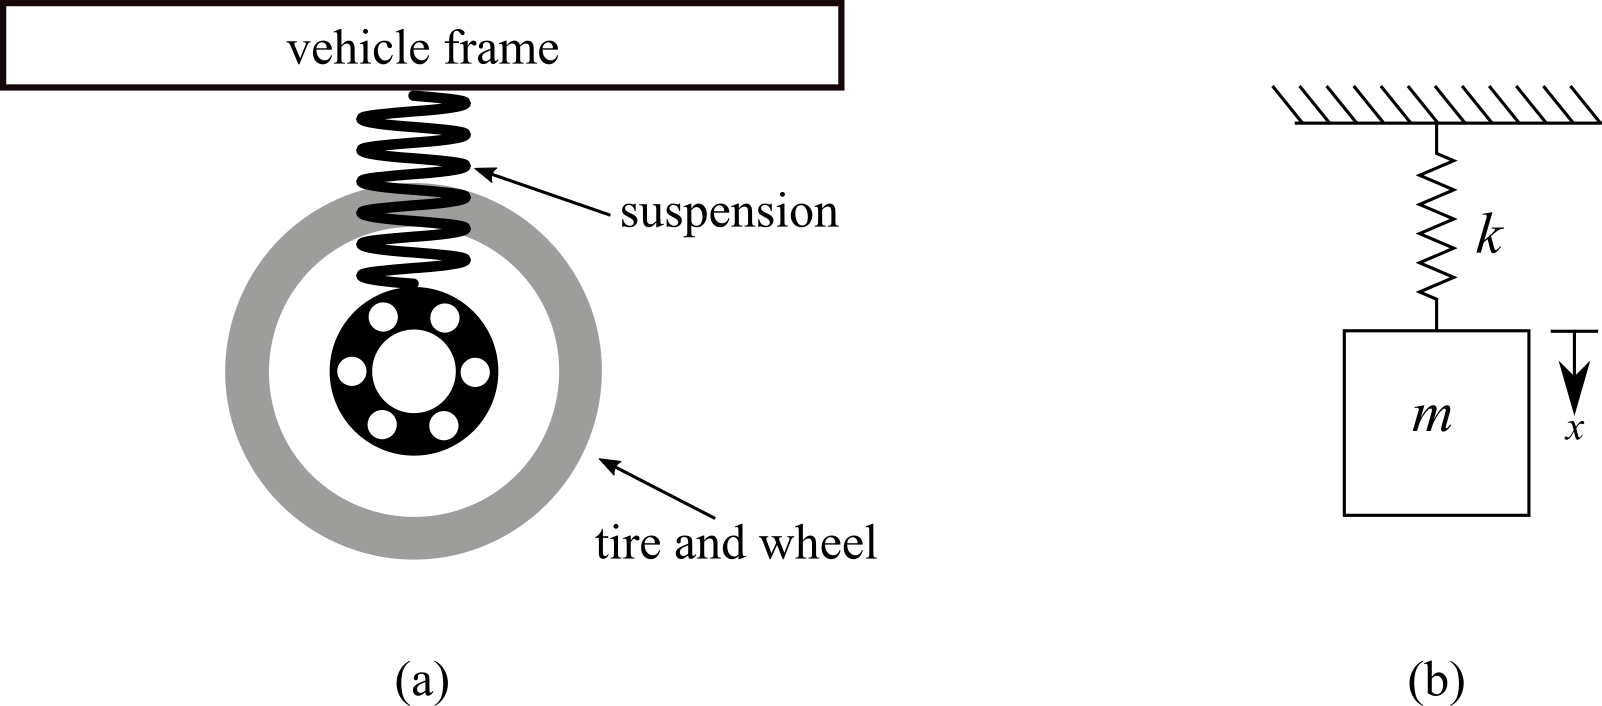
\includegraphics[]{../figures/Vehicle_wheel_undamped.png}
					\caption{Modeling of a vehicle wheel, tire, and suspension showing: (a) Graphical representation; and (b) a spring-mass model.}
					\label{fig:vehicle_wheel_undamped}
				\end{figure}				
				
				\noindent\textbf{Solution:} 

				Considering:
				\begin{equation}
					\omega_\text{n} = \sqrt{\frac{k}{m}}
				\end{equation}
				therefore, $k=m\omega_\text{n}^2=(300$ $\text{kg})(10$ $\text{rad/s})^2=30$ KN/m. 
	
			\end{example}
		
		\begin{example}		

			\textbf{Calculating Natural Frequency}

			\noindent 
				Consider the following 1-DOF system, where $k = 857.8$ N/m and $m=49.2\times10^{-3}$ kg, and calculate the natural frequency in rad/s and Hz. Also, find the period of oscillations and the maximum displacement if the spring is initially displaced $10$ mm with no initial velocity.  	
				\begin{figure}[H]
					\centering
					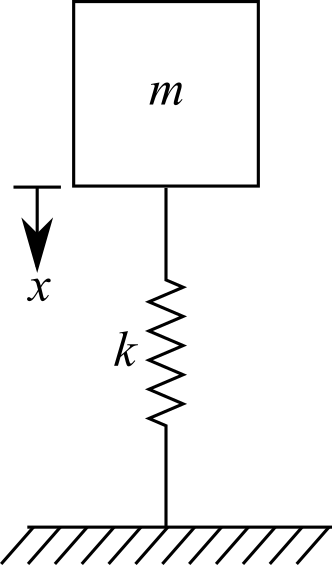
\includegraphics[]{../figures/1-DOF-spring_mass_vertical.png}
					\caption{1-DOF spring-mass system.}
				\end{figure}		
	
				\noindent\textbf{Solution:} 

				\begin{equation}
					\omega_\text{n} = \sqrt{\frac{k}{m}}= \sqrt{\frac{857.8}{49.2\times10^{-3}}} = 132 \hspace{1ex}\text{rad/sec}
				\end{equation}	
				In Hz, this is:
				\begin{equation}
					f_n = \frac{\omega_\text{n}}{2\pi} = 21 \hspace{1ex}\text{Hz}
				\end{equation}						
				The period is:
				\begin{equation}
					T = \frac{2\pi}{\omega_\text{n}} = 0.0476 \hspace{1ex}\text{s}
				\end{equation}					
				The maximum displacement will happen when sin($\omega_\text{n}t+\phi$)$=0$, therefore, the value of $A$ is the maximum displacement. For an undamped system, $	A = \frac{\sqrt{\omega_\text{n}^2x_0^2+v_0^2}}{\omega_\text{n}}$,  
	
	
				\begin{equation}
					A = \frac{\sqrt{\omega_\text{n}^2x_0^2+v_0^2}}{\omega_\text{n}} = \frac{\sqrt{132^2 0.01 ^2+0^2}}{132}=0.01 \hspace{1ex}\text{m}
				\end{equation}
	
			\end{example}

	\subsection{General Solution for Vibrating Systems}

		The EOM for a vibrating system has many solutions and can be expressed in various forms including a general solution. These forms offer different mathematical approaches to solve the same 1-DOF spring-mass system and relate to each other through Euler's equations.
				
		\begin{review}

			\textbf{Complex Plane}

			\noindent Vibration analysis uses complex numbers to solve the EOM's differential equation. In this text the imaginary number is termed $j$ (sometimes referred to as $i$): such that:
			
			\begin{equation}
				j = \sqrt{-1}
			\end{equation}		
			and:	 
			\begin{equation}
				j^2 = -1
			\end{equation}	
			A general complex number, $x$, can be expressed as:
			\begin{equation}
				x=a+bj
			\end{equation}			 	
			here, $a$ is referred to as the real number and $b$ is the imaginary part of the number $x$. Such complex numbers can be represented in the complex plane, also called an Argand plot. The absolute value or modules is defined as $|x|$ presented on the complex plot. 
			
			\begin{figure}[H]
				\centering
				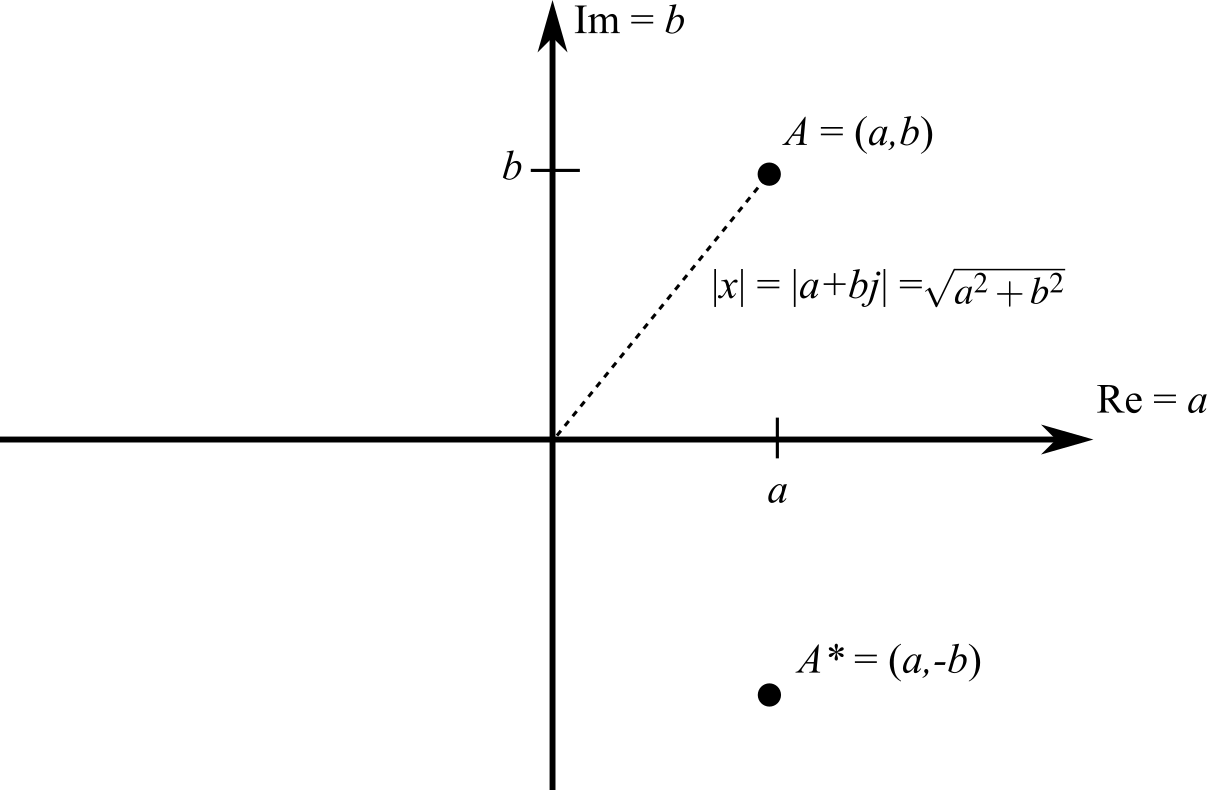
\includegraphics[]{../figures/complex_plane.png}
				\caption{A conjugate pair of numbers ($A$ and $A*$) represented on the complex plane.}
			\end{figure}
					
			$A$ and $A^*$ prime are complex conjugate pairs. In mathematics, the complex conjugate of a complex number is the number with an equal real part and an imaginary part equal in magnitude but opposite in sign. In other words, a conjugate pair is $a + bj$ and $a - bj$.  
			
			\definitionbox{con�ju�gate (adjective)}{Coupled, connected, or related.}

		\end{review}			
		\begin{review}
		
			\textbf{Euler's Formula}

			\noindent Euler's (pronounced oy-ler) formula, is a mathematical formula in complex analysis that establishes the fundamental relationship between the trigonometric functions and the complex exponential function. Euler's formula states that for any real number $x$,
			\begin{equation}
				e^{j\psi} = \text{cos}(\psi) + j \text{sin}(\psi)
			\end{equation}		
			where $j=\sqrt{-1}$. This equation can also be expressed as:
			\begin{equation}
				e^{-j\psi} = \text{cos}(\psi) - j \text{sin}(\psi)
			\end{equation}	
			This can be expressed in terms of polar coordinates as:				
			\begin{figure}[H]
				\centering
				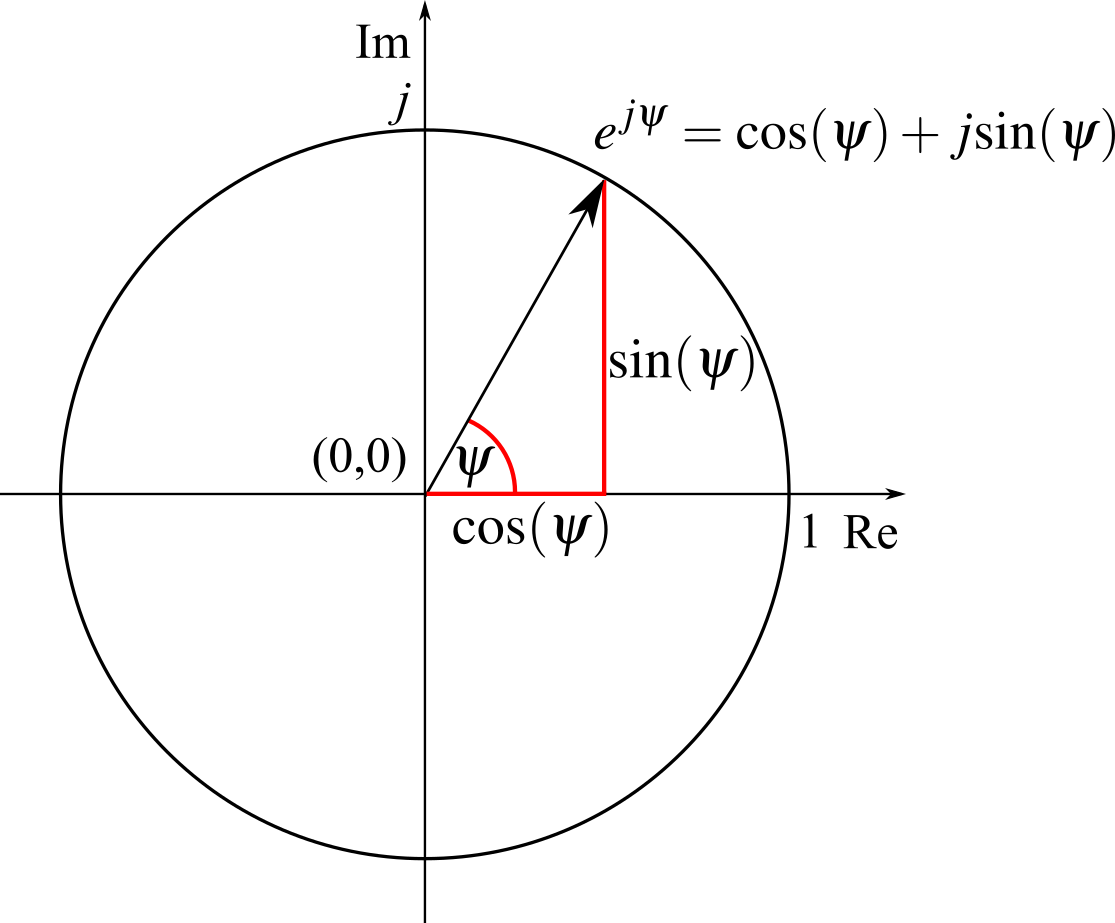
\includegraphics[]{../figures/Eulers_formula.png}
				\caption{Euler's formula illustrated on the unit circle in the complex plane.}
			\end{figure}

			\begin{figure}[H]
				\centering
				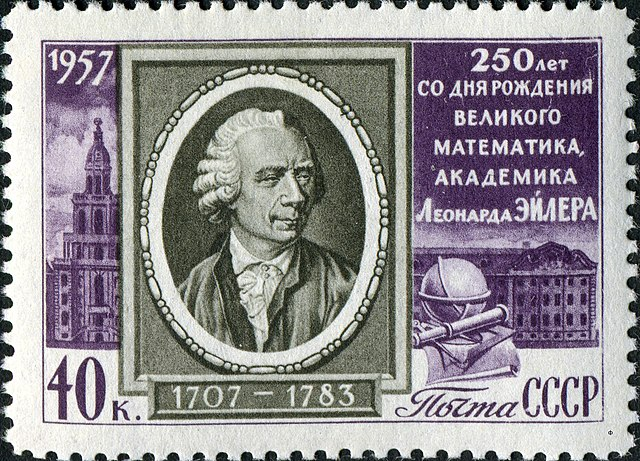
\includegraphics[width=4in]{../figures/Leonhard_Euler}
				\caption{A Soviet Union stamp from 1957 with a Portrait of Leonhard Euler who worked in various branches of the Imperial Russian Academy of Sciences and Imperial court during his lifetime \protect\footnotemark[1].}
			\end{figure}
						
			Euler's formula is named after the Swiss engineer and mathematician Leonhard Euler (1707-1783), who among other things popularized the use of the Greek letter $\pi$ to denote the ratio of a circle's circumference to its diameter, wast the first to use the expression $f(x)$ to denote a function, and correctly defining the base of the natural logarithm $e$; which is now known as Euler's number. While Euler developed ``Euler's formula'' in 1748, it was not used to describe points in a complex for another 50 years when the Danish-Norwegian mathematician and cartographer Caspar Wessel presented to the Danish Academy in 1797  \protect\footnotemark[2].
			

			\footnotetext[1]{Post of the USSR, Public domain, via Wikimedia Commons}  
			\footnotetext[2]{Whittaker, Edmund Taylor, and George Neville Watson. A course of modern analysis: an introduction to the general theory of infinite processes and of analytic functions; with an acount of the principal transcendental functions. University Press, 1927.}  
		
		\end{review}
		
		\subsubsection{Formulating the General Solution for a 1-DOF Spring-Mass System}
			We can also solve the following EOM as an elementary differential equation:
			\begin{equation}
				m\ddot{x}+kx=0
			\end{equation}		
			in a more analytical manner using the theory of elementary differential equations. To do this the form: 
			\begin{equation}
				x(t) = ae^{\lambda t}
			\end{equation}
			is assumed, where $a$ and $t$ are nonzero constants that need to be determined. Using successive differentiation, the assumed solution becomes:
			\begin{equation}
				\dot{x}(t) = \lambda ae^{\lambda t}
			\end{equation}
			and 
			\begin{equation}
				\ddot{x}(t) = \lambda^2 ae^{\lambda t}
			\end{equation}
			therefore, $m\ddot{x}(t) + kx(t) = 0$ becomes:
			\begin{equation}
				m \lambda^2 ae^{\lambda t}  + k ae^{\lambda t} = 0
			\end{equation}
			Next, the above expressions is divide by $ae^{\lambda t}$ to obtain the characteristic equation:
			\begin{equation}
				m \lambda^2 + k = 0
			\end{equation}
			This can be done because $ae^{\lambda t}$ is never zero, therefore, the expression is never divided by zero. The quadratic formula gives us:
			\begin{equation}
				\lambda = \pm \sqrt{-\frac{k}{m}} = \pm \sqrt{\frac{k}{m}}j = \pm \omega_\text{n} j
			\end{equation} 
			remember that $\omega_\text{n} = \sqrt{\frac{k}{m}}$. Notice that the $\pm$ tells us there are two solutions to this problem. So, putting $\lambda$ back into the assumed solution results in two solutions (one positive, one negative):   
			\begin{equation}
				x(t) = a_1e^{+\omega_\text{n} j t}
			\end{equation}
			and 
			\begin{equation}
				x(t) = a_2e^{-\omega_\text{n} j t}
			\end{equation}
		
			As these solutions only consider, and are only valid for, linear systems; the sum of the solutions is also a solution. This simplification results in:
			\begin{equation}
				x(t) = a_1e^{+\omega_\text{n} j t} + a_2e^{-\omega_\text{n} j t}
			\end{equation}
			where $a_1$ and $a_2$ are constants of integration that scale the unit Euler's vector. The positive and negative values in the exponent indicate that the terms are a conjugate pair.

			\begin{review}
				
				\textbf{Superposition of Linear Systems}

				\noindent In linear algebra, the principle of superposition is a fundamental characteristic of linear systems. It states that if $x_1$ and $x_2$ are solutions to a linear system $Ax = b$, where $A$ is a matrix and $b$ is a vector, then any linear combination of these solutions is also a solution to the system. 
				
				Mathematically, if $Ax_1 = b$ and $Ax_2 = b$, then for any scalars $\alpha$ and $\beta$, the vector $\alpha x_1 + \beta x_2$ is also a solution. This can be demonstrated as:
				\begin{equation}
					A(\alpha x_1 + \beta x_2) = \alpha Ax_1 + \beta Ax_2 = \alpha b + \beta b = (\alpha + \beta)b
				\end{equation}
				This principle allows for the construction of the general solution to a linear system.
			\end{review}		

			
			
			\begin{example}
				\textbf{Equivalences of Mathematical Vibration Models}

				\noindent 

				Show that $	x(t) = a_1e^{+\omega_\text{n} j t} + a_2e^{-\omega_\text{n} j t}$ is equal to $A\text{sin}(\omega_\text{n} t +\phi)$. \\
				
				\noindent\textbf{Solution:} 

				\noindent This equation was derived using Euler's formula and it can be shown that this equation is equivalent to the $A\text{sin}(\omega_\text{n}+\phi)$. To recover the previously assumed solution, the knowledge that $a_1$ and $a_2$ are complex congregate pairs and as such the magnitude can be expressed as $a_1=a_2$ is leveraged. Using Euler's polar notation, $a_1$ and $a_2$ can be expressed as 
				\begin{equation}
					a_1 = a_2 = ae^{j\psi}
				\end{equation}	
				where $a$ and $\psi$ are real numbers, the equation becomes:		
				\begin{equation}
					x(t) = ae^{j(\omega_\text{n} t+\psi)} + ae^{-j(\omega_\text{n} t+\psi)}
				\end{equation}			
				this becomes:
				\begin{equation}
					x(t) = a(e^{j(\omega_\text{n} t+\psi)} + e^{-j(\omega_\text{n} t+\psi)})
				\end{equation}				
				
				Remembering Euler's equations from before, this becomes:
				\begin{equation}
					x(t) = a\big(\text{cos}(\omega_\text{n} t+\psi) + j \text{sin}(\omega_\text{n} t+\psi) + \text{cos}(\omega_\text{n} t+\psi) - j \text{sin}(\omega_\text{n} t+\psi)\big)
				\end{equation}				
				combining the ``cos'' terms and canceling out the ``sin'' terms this becomes:
				\begin{equation}
					x(t) = 2a \cdot \text{cos}(\omega_\text{n} t+\psi)
				\end{equation}						
				This is equivalent to $	{x}(t) = A\text{sin}(\omega_\text{n} t + \phi)$ considering that $A=2a$ and knowing sin($\phi$) = cos($\phi + \psi$). To expand, this is because the sin and cos are only differentiated by a phase shift. 			
			\end{example}

			
			Next, a general solution for the EOM is obtained. Using the previous solution:
			\begin{equation}
				x(t) = a_1e^{+\omega_\text{n} j t} + a_2e^{-\omega_\text{n} j t}
			\end{equation}			
			we can expand this into the form: 
			\begin{equation}
				x(t) = a_1\big(\text{cos}(\omega_\text{n} t) + j \text{sin}(\omega_\text{n} t)\big) + a_2\big(\text{cos}(\omega_\text{n} t) - j \text{sin}(\omega_\text{n} t)\big)
			\end{equation}
			using trigonometric functions. This equates to:
			\begin{equation}
				x(t) = (a_1+a_2) \cdot \text{cos}(\omega_\text{n} t) + (a_1-a_2)j \cdot \text{sin}(\omega_\text{n} t)
			\end{equation}			
			As $x(t)$ is always real, $A_1$ and $A_2$ can be defined as:
			\begin{equation}
				A_1 = (a_1+a_2)
			\end{equation}		
			and
			\begin{equation}
				A_2 = (a_1-a_2)j
			\end{equation}	
			Lastly, the general solution is written as:
			\begin{equation}
				x(t) = A_1\text{cos}(\omega_\text{n} t) + A_2\text{sin}(\omega_\text{n} t)
			\end{equation}	
			This is the general solution for the EOM ($m\ddot{x}+kx=0$) of the considered oscillating system where $A_1$ and $A_2$ are defined as:
			\begin{equation}
				A = \sqrt{A_1^2+ A_2^2}
			\end{equation}
			and	
			\begin{equation}
				\phi = \text{tan}^{-1}\bigg(\frac{A_1}{A_2}\bigg)
			\end{equation}		
			These are obtained from a trigonometric relationship, similar to that used before:
			\begin{figure}[H]
				\centering
				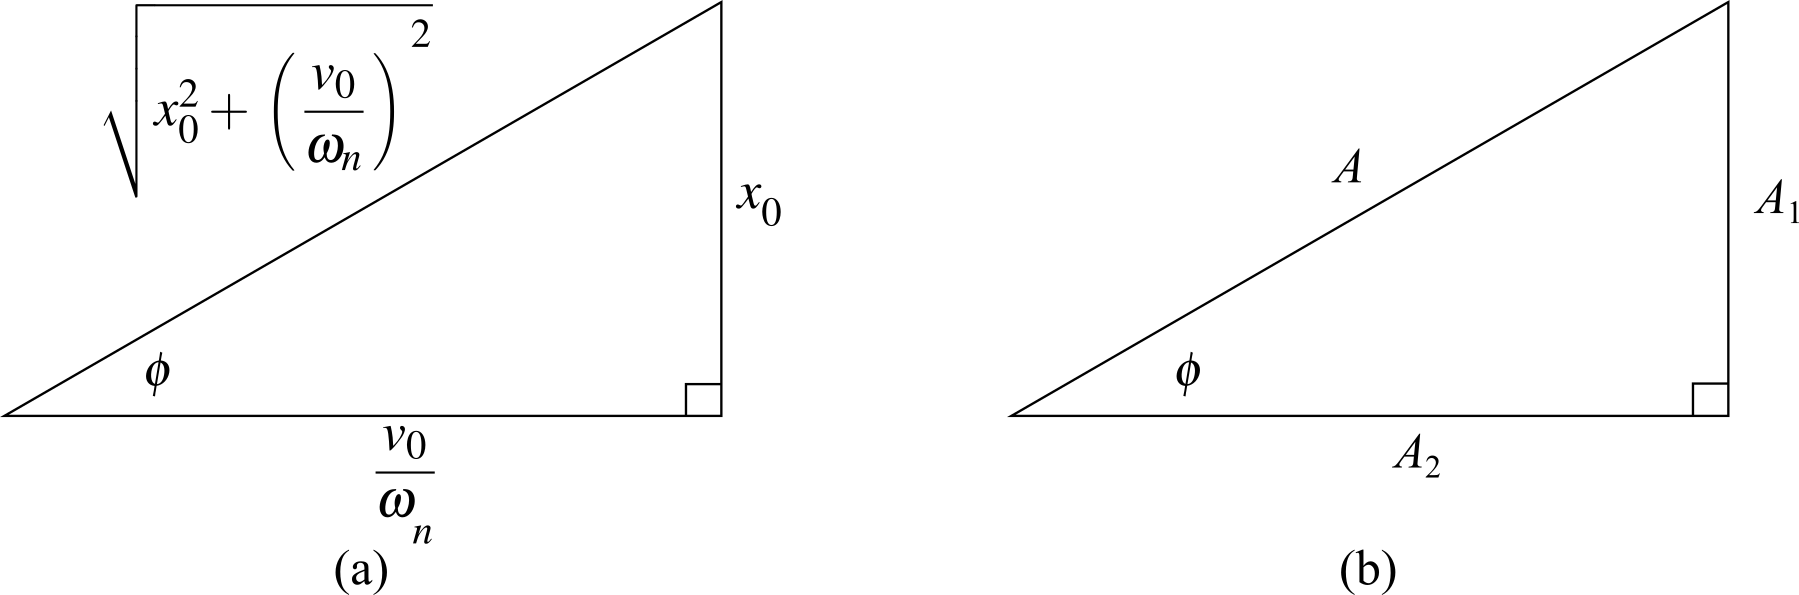
\includegraphics[]{../figures/trigonometric_relationship_undamped_free_general_solution.png}
				\caption{Trigonometric relationship between the initial conditions, amplitude, and phase, for free vibration of a 1-DOF system expressed with: (a) variables for initial conditions; and (b) generic variables $A_{1}$ and $A_{2}$.}
			\end{figure}
			\noindent again, $A$ and $\phi$ are:
			\begin{equation}
				A = \frac{\sqrt{\omega_\text{n}^2x_0^2+v_0^2}}{\omega_\text{n}} = \sqrt{x_0^2+\Bigg(\frac{v_0}{\omega_\text{n}}\Bigg)^2}
			\end{equation}
			\begin{equation}
				\phi = \text{tan}^{-1}\bigg(\frac{x_0\omega_\text{n}}{v_0}\bigg)
			\end{equation}		


			\begin{example}			

				\textbf{Solving for Constants in the General Solution}

				\noindent Using the general solution: 
				\begin{equation}
					x(t) = A_1\text{cos}(\omega_\text{n} t) + A_2\text{sin}(\omega_\text{n} t)
				\end{equation}			
				Calculate the values of $A_1$ and $A_2$ in terms of their initial conditions $x_0$ and $v_0$.
				
				\noindent \textbf{Solution:} 

				\noindent Knowing the following for $x$ and $\dot{x}$:
				\begin{equation}
					x(t) = A_1\text{cos}(\omega_\text{n} t) + A_2\text{sin}(\omega_\text{n} t)
				\end{equation}	
				\begin{equation}
					\dot{x}(t) = -A_1\omega_\text{n}\text{sin}(\omega_\text{n} t) + A_2\omega_\text{n}\text{cos}(\omega_\text{n} t)
				\end{equation}	
				Now apply the initial conditions, $x(0)=0$ and $v(0)=0$, this yields:
				\begin{equation}
					x(0) = x_0 = A_1
				\end{equation}	
				\begin{equation}
					\dot{x}(0)= v_0  =  A_2\omega_\text{n}
				\end{equation}
				Solving for $A_1$ and $A_2$ shows us:
				\begin{equation}
					A_1 = x_0 \text{, and } A_2 = \frac{v_0}{\omega_\text{n}}
				\end{equation}
				thus:
				\begin{equation}
					x(t) = x_0\text{cos}(\omega_\text{n} t) + \frac{v_0}{\omega_\text{n}}\text{sin}(\omega_\text{n} t)
				\end{equation}				
			\end{example}

		\subsubsection{Solution of 1-DOF System in Three Forms}
			Form one, for $m\ddot{x} + kx =0$ subject to nonzero initial conditions can be written as:  		
			\begin{equation}
				x(t) = a_1e^{+\omega_\text{n} j t} + a_2e^{-\omega_\text{n} j t}
			\end{equation}	
			where $a_1$ and $a_2$ are complex terms. Form two is:
			\begin{equation}
				{x}(t) = A\text{sin}(\omega_\text{n} t + \phi)
			\end{equation}
			while form three is:
			\begin{equation}
				x(t) = A_1\text{cos}(\omega_\text{n} t) + A_2\text{sin}(\omega_\text{n} t)
			\end{equation}	
			where $A$, $\phi$, $A_1$, and $A_2$, are all real-valued constants. Each set of constants can be related to each other by:
			\begin{align}
				\label{eq:A_1_and_A_2}
				A = \sqrt{A_1^2+ A_2^2} & \hspace{1.5cm} \phi = \text{tan}^{-1}\bigg(\frac{A_1}{A_2}\bigg) \\
				A_1 = (a_1+a_2) & \hspace{1.5cm} A_2 = (a_1-a_2)j \\
				a_1 = \frac{A_1-A_2j}{2} & \hspace{1.5cm} a_2 = \frac{A_1+A_2j}{2}
			\end{align}
			Which follow from trigonometric identities and Euler's formula. 







	
	\subsection{Damping}
	
	
		The response of a spring-mass system predicts that a system will oscillate indefinitely. However, we know that this is not true from observing real-world solutions. So based on real-world observations and mathematical conveniences, we need to add a term that will remove ``energy'' from the system with time. To do this the idea of the ideal dashpot is introduced. A linear dashpot is diagrammed in figure \ref{fig:linear_dashpot} and is a mechanical device that resists motion via viscous friction and therefore converts the mechanical energy of the system into thermal energy that is dissipated.
		
		\begin{figure}[H]
			\centering
			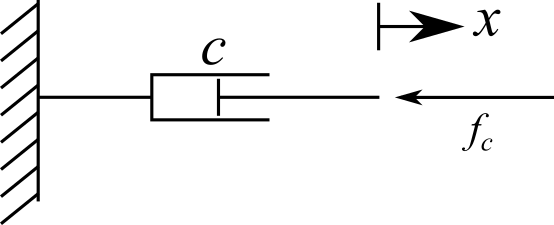
\includegraphics[]{../figures/linear_dashpot.png}
			\caption{Schematic of a liner dashpot showing the damping force ($f_c$) acting in the opposite direction of the displacement ($x$).}
			\label{fig:linear_dashpot}
		\end{figure}
		
		Just as spring forms a physical model of the cause vibration, through its storage and release of energy, a dashpot (sometimes called a damper) forms a physical model for dissipating energy. Dashpots create a resisting or damping force that acts opposite to the direction of travel (as annotated in figure \ref{fig:linear_dashpot}) and is proportional to the velocity. Therefore, the damping forces $f_c$ can be computed as:
		\begin{equation}
			f_c = c \dot{x}
		\end{equation}
		the constant $c$, called the damping coefficient, has the units of kg/s. Dashpots are a mathematical representation of viscous dampers installed in automobiles, aircraft, structures, and other mechanical devices. However, all systems have inherent damping not just systems with physical dampers. The spring-mass system can be used as a representation of real-world systems with inherent damping as demonstrated by the rubber engine mount depicted in figure \ref{fig:rubber_engine_mount}.
		
		
		\begin{figure}[H]
			\centering
			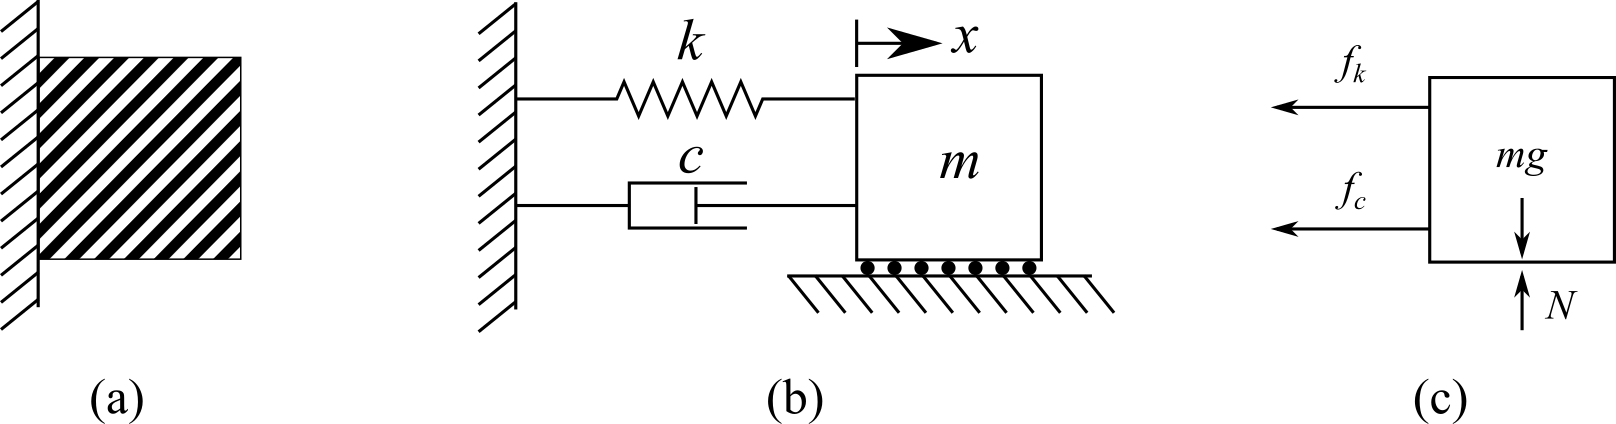
\includegraphics[]{../figures/engine_mount_model.png}
			\caption{Modeling of a rubber engine mount as an spring-dashpot-mass model showing (a) the rubber engine mount; (b) idealized model of the rubber month; and (c) the FBD of the idealized model}
			\label{fig:rubber_engine_mount}
		\end{figure}

		Depending on the amount of damping present in a system, the temporal response of the system will represent itself in various ways, as represented in figure \ref{fig:damping_cases}. To reiterate, an undamped case will oscillate around the equilibrium and does not decay. If a limited amount of damping is present in a system it will oscillate around the equilibrium and slowly decay with time to the equilibrium position, this is termed underdamped. If an excessive amount of damping is present, the system will not oscillate but decay directly to the equilibrium position, this is termed the overdamped case. Lastly, there exists a special case that results in the system converging as quickly as possible to the equilibrium position without oscillations; this case is termed the critically damped case. Furthermore, the amount of damping required to obtain a critically damped system is the damping value between the underdamped and overdamped cases for a specific system. To recap, the key types of damping are:
		
		\begin{itemize}
			\item \textbf{Undamped} - Oscillates about the equilibrium and does not decay.
			\item \textbf{Underdamped} - Oscillates about the equilibrium and slowly decays and is the most common case.
			\item \textbf{Overdamped} - Does not pass the equilibrium position and is a simple decay with no oscillation.
			\item \textbf{Critically damped} - Provides the quickest approach to zero amplitude for a damped oscillator, no oscillation.
		\end{itemize}
		
		
		\begin{figure}[H]
			\centering
			\includegraphics[]{../figures/damping_cases.png}
			\caption{Temporal responses for the three types of damping: underdamped, overdamped, and critically damped.}
			\label{fig:damping_cases}
		\end{figure}

		\begin{vibration_case_study}

			\textbf{Supplemental Damping on Suspension Bridges}

			\noindent Dampers are used to extract energy from systems in an effort to reduce their vibrations. The Author Ravel Junior Bridge in Charleston South Carolina is a cable-stayed bridge over the Cooper River with a main span of 471 m (1,546 feet). The bridge uses two dampers connected to the cables in the middle of the bridge to dissipate excess energy in the cables that would otherwise cause unwanted vibrations from wind, traffic, and seismic activity. The inclusion of these dampers on the bridges is a proactive measure to enhance the bridge's performance, safety, and user experience by reducing the effects of vibrations.
			
		\begin{figure}[H]
			\centering
			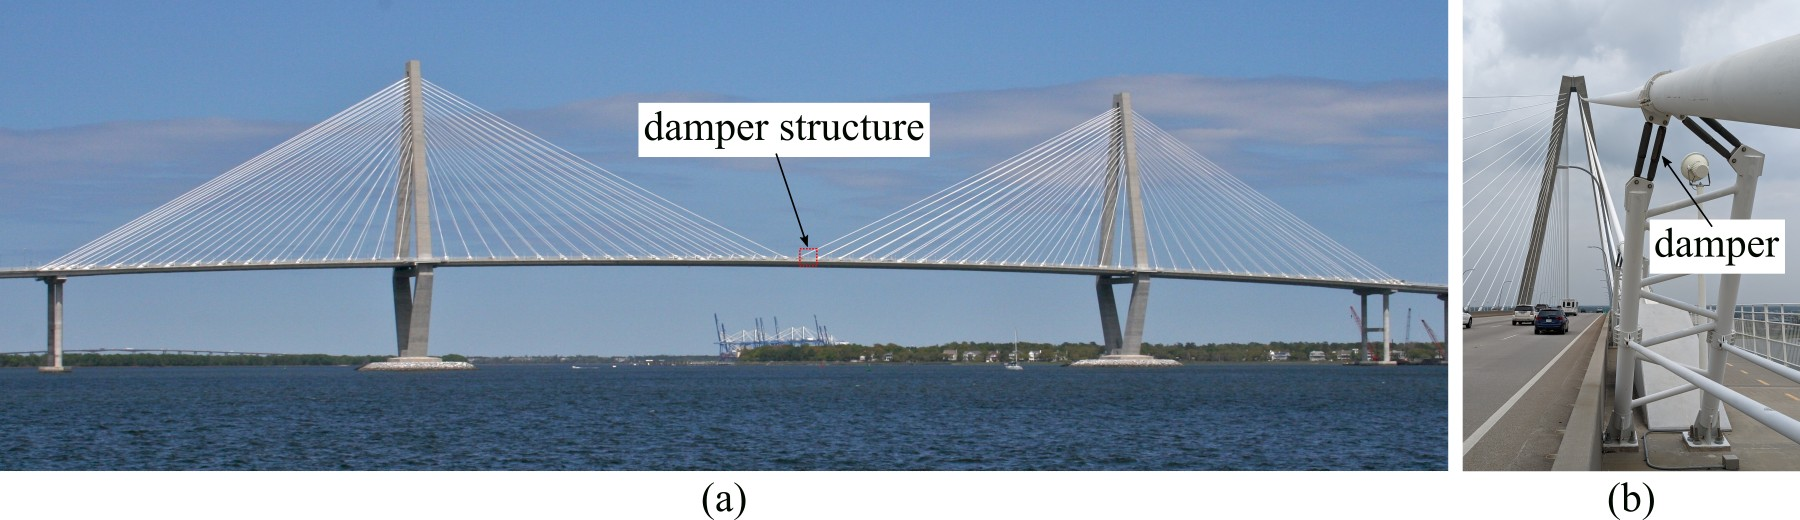
\includegraphics[width=6in]{../figures/Arthur_Ravenel_Jr._Bridge}
			\caption{Dampers installed on the center cables of the Author Ravel Junior Bridge in Charleston South Carolina, showing: (a) the main span of the bridge taken from the water\protect\footnotemark[1] with the damper structure annotated; and (b) close up of the structure that holds the damper.}
				\footnotetext[1]{original un-annotated image by bbatsell, CC BY-SA 2.5 $<$https://creativecommons.org/licenses/by-sa/2.5$>$, via Wikimedia Commons}
		\end{figure}		
		\end{vibration_case_study}
			
		\subsubsection{Modeling Vibrating Systems with Damping}
				
			The spring-mass system of Chapter 1 can be expanded to a spring-dashpot-mass system that considers the damping component of the system. A mathematical model of the spring-dashpot-mass system can be developed for the case present in figure \ref{fig:1-DOF-mass_horizontal_damping_FBD}. Using the FBD for the system, it can conclude that the EOM for this system:
			\begin{figure}[H]
				\centering
				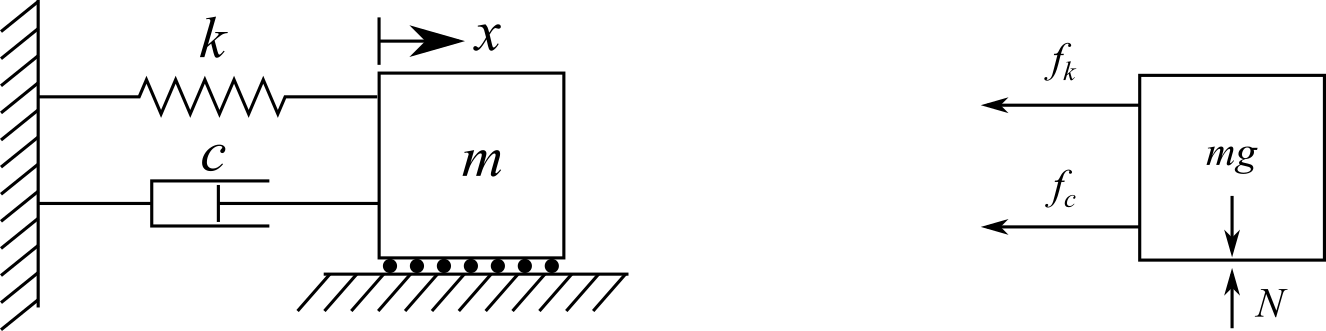
\includegraphics[]{../figures/1_DOF_spring_dashpot_mass_horizontal_FBD.png}
				\caption{Spring-dashpot-mass model showing: (a) a schematic of the system; and (b) the FBD of the system. }
				\label{fig:1-DOF-mass_horizontal_damping_FBD}
			\end{figure}			
			\noindent is:
			\begin{equation}
				m\ddot{x}(t) = - f_c - f_k
			\end{equation}
			Rearranging into standard form and concerting forces into parameters $c$ and $k$ results in:
			\begin{equation}
				m\ddot{x}(t) + c \dot{x}(t) + kx(t) = 0
			\end{equation}
			This system is subject to the same initial conditions as before, $x(0) = x_0$ and $\dot{x}(0) = v_0$. Again, choosing to model it this way for convinces, so let's solve it in a similar manner to the EOM without damping. Again, assume the solution:
			\begin{equation}
				x(t) = ae^{\lambda t}
			\end{equation}
			here, $a$ and $t$ are nonzeros constants that need to be determined.  Using successive differentiation, we get:
			\begin{equation}
				\dot{x}(t) = \lambda ae^{\lambda t}
			\end{equation}
			and 
			\begin{equation}
				\ddot{x}(t) = \lambda^2 ae^{\lambda t}
			\end{equation}
			therefore, $m\ddot{x} + c\dot{x} + kx = 0$ becomes:
			\begin{equation}
				m \lambda^2 ae^{\lambda t}  +c\lambda ae^{\lambda t} + k ae^{\lambda t} = 0
			\end{equation}
			Now we divide by $ae^{\lambda t}$ to obtain the \textbf{characteristic equation}:
			\begin{equation}
				m \lambda^2 + c\lambda + k = 0
			\end{equation}
			We can do this because $ae^{\lambda t}$ is never zero, therefore, we never divide by zero. The quadratic formula gives us:
			\begin{equation}
				\lambda_{1,2} = \frac{-c \pm \sqrt{c^2-4km}}{2m}  = \frac{-c}{2m} \pm \frac{1}{2m}\sqrt{c^2-4km}
			\end{equation}
			Some key points from this equation:
			\begin{itemize}
			\item The $\pm$ tells us there are two solutions to this problem
			\item if $c^2-4km<0$, system is Underdamped, solutions are complex conjugate pairs 
			\item if $c^2-4km=0$, system is critically damped, solutions are equal negative real numbers 
			\item if $c^2-4km>0$, system is Overdamped, solutions are distinct negative real numbers 
			\end{itemize}
			From this, we can see that $c^2-4km=0$ is a special value, let us define a value for $c$ that will give us this critical damping number. We will call it the \textbf{critical damping coefficient} ($c_{\text{cr}}$). So setting the equation as:
			\begin{equation}
				c_{\text{cr}}^2-4km = 0
			\end{equation}
			giving us: 
			\begin{equation}
				c_{\text{cr}}^2 = 4km
			\end{equation}		
			next, we can derive the function:
			\begin{equation}
				c_{\text{cr}} = 2\sqrt{km} = 2\bigg(\frac{\sqrt{m}}{\sqrt{m}}\bigg)\sqrt{km} = 2m\omega_\text{n}
			\end{equation}			
			remember that $\omega_\text{n} = \sqrt{\frac{k}{m}}$ for an undamped system. Next, we generate a non-dimensional number ($\zeta$), pronounced `zeta' that will allow us to distinguish between different types of damping. $\zeta$ is called the \textbf{critical damping ratio}.
			\begin{equation}
				\zeta = \frac{c}{c_{\text{cr}}} = \frac{c}{2\sqrt{km}} = \frac{c}{2m\omega_\text{n}}
			\end{equation}				
			Now if we put the $\zeta$ back into the characteristic equation and resolve using the quadratic equation we get: 
			\begin{equation}
				\lambda_{1,2} = -\zeta\omega_\text{n} \pm \omega_\text{n} \sqrt{\zeta^2-1}
			\end{equation}
			From this equation, it becomes clear that $\zeta$ determines whether the roots are complex or real, this, in turn, determines the nature of the response of the structure. Listing the possible responses we get:
			\begin{table}[h!]
				\centering
				\begin{tabular}{lccc}
					\toprule
					damping case & critical damping ratio & radicand & solutions  \\ \midrule
					under damped &  $0<\zeta<1$ & $c^2-4km<0$ & complex conjugate pairs \\
					critically damped & $\zeta=1$ & $c^2-4km=0$ & equal negative real numbers \\
					over damped & $1<\zeta$  & $c^2-4km>0$ & distinct negative real numbers \\ \bottomrule
				\end{tabular}
			\end{table}
			For each damping case, we will have a different solution to the problem. 
					
		\subsubsection{Modeling Underdamped Motion}
		
 			In the case that $0<\zeta<1$, a complex conjugate pair of roots are the solutions to the characteristic equation after pulling out a $\sqrt{-1}$:
			\begin{equation}
				\lambda_{1} = -\zeta\omega_\text{n} + \omega_\text{n} \sqrt{1-\zeta^2}j
			\end{equation} 			
			and:
			\begin{equation}
				\lambda_{2} = -\zeta\omega_\text{n} - \omega_\text{n} \sqrt{1-\zeta^2}j
			\end{equation} 
			Where the $j$ is pulled out because:
			\begin{equation}
				\sqrt{1-\zeta^2}j = \sqrt{(1-\zeta^2)(-1)} = \sqrt{\zeta^2-1}
			\end{equation} 							
			Next, let us ``arbitrarily'' define:
			\begin{equation}
				\omega_\text{d} = \omega_\text{n}\sqrt{1-\zeta^2}
			\end{equation} 	
			where $\omega_\text{d}$ is the \textbf{damped natural frequency}. Therefore, the equations become:
			\begin{equation}
				\lambda_{1} = -\zeta\omega_\text{n} + \omega_\text{d}j
			\end{equation} 			
			and:
			\begin{equation}
				\lambda_{2} = -\zeta\omega_\text{n} - \omega_\text{d}j
			\end{equation} 	
			Again, we have two solutions to a linear problem, so we can combine these into one solution and insert $\lambda$ into the assumed solution $ae^{\lambda t}$ to obtain:
			\begin{equation}
				x(t) = a_1e^{-\zeta\omega_\text{n}t + \omega_\text{d}tj} + a_2e^{-\zeta\omega_\text{n}t - \omega_\text{d}tj} 
			\end{equation} 			
			where $a_1$ and $a_2$ are complex valued constants. This can now be simplified into:	
			\begin{equation}
				x(t) = e^{-\zeta\omega_\text{n}t}(a_1e^{\omega_\text{d}tj} + a_2e^{-\omega_\text{d}tj}) 
			\end{equation} 

			Using Euler's equations, (same as before) and choosing:
			\begin{equation}
				A_1=(a_1-a_2)j
			\end{equation} 	
			and
			\begin{equation}
				A_2=(a_1+a_2)
			\end{equation} 		
			Note that the $A_1$ and $A_2$ defined here are the reverse of those defined in Eq.~\ref{eq:A_1_and_A_2}. This is done to allow the general form to be in the same format as before, however, assuming the same $A_1$ and $A_2$ would not change the final solution expressed below. The general form of this solution is then:
			\begin{equation}
				x(t) = e^{-\zeta\omega_\text{n}t}\big(A_1\text{sin}(\omega_\text{d}t) + A_2\text{cos}(\omega_\text{d}t)\big)
			\end{equation} 	
			Recall that for undamped 1-DOF systems we showed 
			\begin{equation}
				x(t) = A\text{sin}(\omega_\text{n}t + \phi) = A_1\text{sin}(\omega_\text{n}t) + A_2\text{cos}(\omega_\text{n}t)
			\end{equation} 	
			As $e^{-\zeta\omega_\text{n}t}$ accounts for the damping, our current solution becomes:
			\begin{equation}
				x(t) = Ae^{-\zeta\omega_\text{n}t}\text{sin}(\omega_\text{d}t + \phi) 
			\end{equation} 		

			Now that we have $x$ and $\dot{x}$, we can solve for the boundary conditions $x_0$ and $v_0$ by setting $t=0$, we get:
			\begin{equation}
				x(0)=x_0 = A\text{sin}(\phi) 
			\end{equation} 			
			and taking the directive of $x(t)$ using the product rule (fg)'= f'g+fg', we get:
			\begin{equation}
				\dot{x}(t) = -\zeta\omega_\text{n}Ae^{-\zeta\omega_\text{n}t}\text{sin}(\omega_\text{d}t + \phi) + Ae^{-\zeta\omega_\text{n}t}\omega_\text{d}\text{cos}(\omega_\text{d}t + \phi) 
			\end{equation} 
			\begin{equation}
				\dot{x}(0) =v_0= -\zeta\omega_\text{n}A\text{sin}(\phi) + A\omega_\text{d}\text{cos}(\phi) 
			\end{equation} 
			a simplification can be made to the prior equation by letting $A=x_0/\text{sin}(\phi)$. This gives us the equation:
			\begin{equation}
				\dot{x}(0) =v_0= -\zeta\omega_\text{n}\bigg(\frac{x_0}{\text{sin}(\phi)}\bigg)\text{sin}(\phi) + \bigg(\frac{x_0}{\text{sin}(\phi)}\bigg)\omega_\text{d}\text{cos}(\phi) 
			\end{equation} 			
			that can be simplified to:
			\begin{equation}
				\dot{x}(0) = v_0 = -\zeta\omega_\text{n}x_0 + x_0\omega_\text{d}\text{cot}(\phi) 
			\end{equation} 	
			The above equation related $v_0$ to $\phi$ using terms that are known for a giving system ($\zeta,\, \omega_\text{n},\, x_0 \text{, and }\omega_\text{d} $). Therefore, this expression can be used to solve for $\phi$:
			\begin{equation}
				\text{cot}(\phi) = \frac{v_0 +\zeta\omega_\text{n}x_0}{x_0\omega_\text{d}} 
				\label{eq:underdamped_phi}
			\end{equation} 	
			and as $\tan(\phi) = 1/\text{cot}(\phi)$: 
			\begin{equation}
				\phi = \tan^{-1}\Bigg(\frac{x_0\omega_\text{d}}{v_0+\zeta\omega_\text{n}x_0}\Bigg)
			\end{equation} 				
			Thereafter, we can solve for $A$ considering the fact that we sent $A=x_0/\text{sin}(\phi)$. Using the trigonometric relationship between expressed in equation \ref{eq:underdamped_phi} and visualized in figure \ref{fig:trigonometric_relationship_underdamped}:
			\begin{figure}[H]
				\centering
				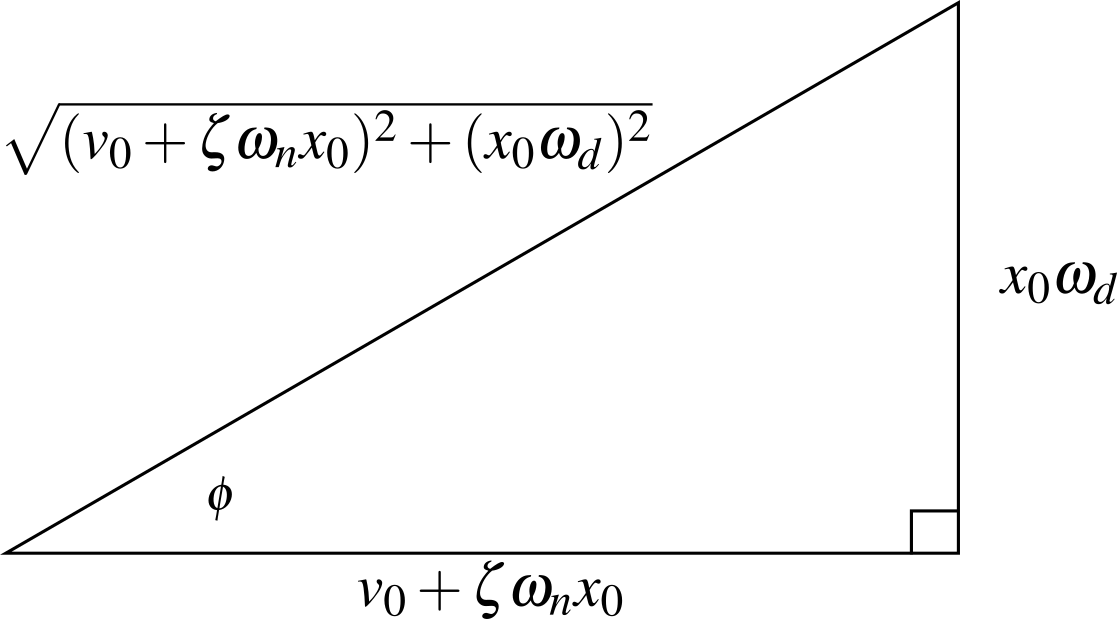
\includegraphics[]{../figures/trigonometric_relationship_underdamped.png}
				\caption{Trigonometric relationship between the initial conditions ($x_0$ and $v_0$), amplitude $A$, and phase $\phi$ for underdamped motion of a 1-DOF system.}
				\label{fig:trigonometric_relationship_underdamped}
			\end{figure}
			\noindent we show that $\text{sin}(\phi)$ can be expressed as: 
			\begin{equation}
				\text{sin}(\phi) = \frac{x_0\omega_\text{d}}{\sqrt{(v_0+\zeta\omega_\text{n}x_0)^2 + (x_0\omega_\text{d})^2}}
			\end{equation} 	
			and applying $A=x_0/\text{sin}(\phi)$ we get:
			\begin{equation}
				A = \frac{\sqrt{(v_0+\zeta\omega_\text{n}x_0)^2 + (x_0\omega_\text{d})^2}}{\omega_\text{d}} = \sqrt{x_0^2 + \Bigg( \frac{v_0 + \zeta \omega_\text{n} x_0}{\omega_\text{d}}\Bigg)^2}
			\end{equation} 								
			Finally, collecting all of our important equations:
			\begin{itemize}
			\item Critical damping coefficient: $c_{\text{cr}} = 2\sqrt{km} = 2m\omega_\text{n}$
			\item Damping ratio: $	\zeta = \frac{c}{c_{\text{cr}}} = \frac{c}{2\sqrt{km}} = \frac{c}{2m\omega_\text{n}}$
			\item Damped natural frequency: $\omega_\text{d} = \omega_\text{n}\sqrt{1-\zeta^2}$
			\item Solution for underdamped system: $x(t) = Ae^{-\zeta\omega_\text{n}t}\text{sin}(\omega_\text{d}t + \phi)$, where: \begin{align*}
						A = \frac{\sqrt{(v_0+\zeta\omega_\text{n}x_0)^2 + (x_0\omega_\text{d})^2}}{\omega_\text{d}} & \hspace{1.5cm} \phi = \text{tan}^{-1}\Bigg(\frac{x_0\omega_\text{d}}{v_0+\zeta\omega_\text{n}x_0}\Bigg) 
						\end{align*}
			\end{itemize}

			\begin{figure}[H]
				\centering
				\includegraphics[]{../figures/under_damped_various_initial_conditions.png}
				\caption{Four example responses for an underdamped 1-DOF system  ($\zeta=0.142$) with various initial conditions.}
			\end{figure}

		\begin{example}				

			\noindent \textbf{Solving for Percent Damping} 

			\noindent Consider the following 1-DOF system, where $k = 857.8$ N/m, $c=7.8$ kg/s, and $m=49.2\times10^{-3}$ kg, calculate the percentage of damping and the damped frequency in rad/s and Hz.
			\begin{figure}[H]
				\centering
				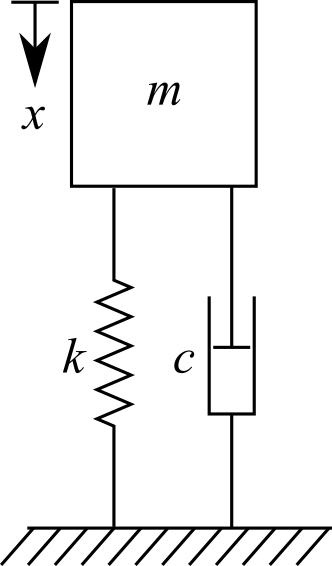
\includegraphics[]{../figures/1_DOF_spring_dashpot_mass_vertical.png}
				\caption{1-DOF spring-dashpot-mass system.}
			\end{figure}		

			\noindent\textbf{Solution:} 
			
			\noindent Calculate the undamped frequency:
			\begin{equation}
				\omega_\text{n} = \sqrt{\frac{k}{m}}= \sqrt{\frac{857.8}{49.2\times10^{-3}}} = 132 \hspace{1ex}\text{rad/s}
			\end{equation}	
			The systems critical damping value:
			\begin{equation}
				c_{\text{cr}} = 2\sqrt{km}= 2\sqrt{k = 857.8 \cdot 49.2\times10^{-3}} = 12.993 \hspace{1ex}\text{kg/s}
			\end{equation}		
			And the critical damping ratio:
			\begin{equation}
				\zeta = \frac{c}{c_{\text{cr}}} = \frac{7.8}{12.993} = 0.600
			\end{equation}				
			This can be expressed as 60\% damped, this is an underdamped system, and the system will oscillate. Now we can calculate the damped frequency:
			\begin{equation}
				\omega_\text{d} = \omega_\text{n}\sqrt{1-\zeta^2} = \omega_\text{n}\sqrt{1-0.600^2} = 105.6 \hspace{1ex}\text{rad/s}
			\end{equation}		
			Therefore, the system oscillates at 105.6 rad/sec or 16.81 Hz
		\end{example}

		\begin{example}

			\noindent \textbf{Solving for the Damping Case} 

			\noindent For a damped one DOF system where $m$, $c$, and $k$ are known to be $m$ = 1 kg, $c$ = 2 kg/s, and $k$ = 10 N/m. Calculate the value of $\zeta$ and $\omega_\text{n}$. Is the system overdamped, underdamped, or critically damped?	

			\noindent\textbf{Solution:} 
						
			The natural frequency is calculated as
			\begin{equation}
				\omega_\text{n} = \sqrt{\frac{k}{m}} = \sqrt{\frac{10}{1}} = 3.16 \hspace{1ex} \text{rad/s}
			\end{equation}
			The damping can be calculated as:
			\begin{equation}
				\zeta = \frac{c}{2\omega_\text{n} m} = \frac{2}{2\Big(\sqrt{\frac{10}{1}}\Big)(1)} = \frac{1}{\sqrt{10}} = 0.316 
			\end{equation}
			So the damped natural frequency is equal to:
			\begin{equation}
				\omega_\text{d} = \omega_\text{n}\sqrt{1-\zeta^2} =  \sqrt{10}\sqrt{1-\bigg(\frac{1}{\sqrt{10}}\bigg)^2} = 3 \hspace{1ex} \text{rad/s}
			\end{equation}			
			As $0<\zeta<1$ the system is underdamped. 			
		\end{example}

		\begin{example}

			\noindent \textbf{Off Orthogonal Stiffness} 

			\noindent Figure~\ref{fig:rubber_mounted_mass_with_spring} shows an industrial device consisting of a mass isolated from its fixtures by two rubber dampers and an offset spring with an angle $\alpha$. Provide an estimate of the system's damped natural frequency in the vertical direction.	Assume the rubber dampers add damping and only negligible stiffness to the system and that the spring is long enough such that the angles remain constant. 	
			\begin{figure}[H]
				\centering
				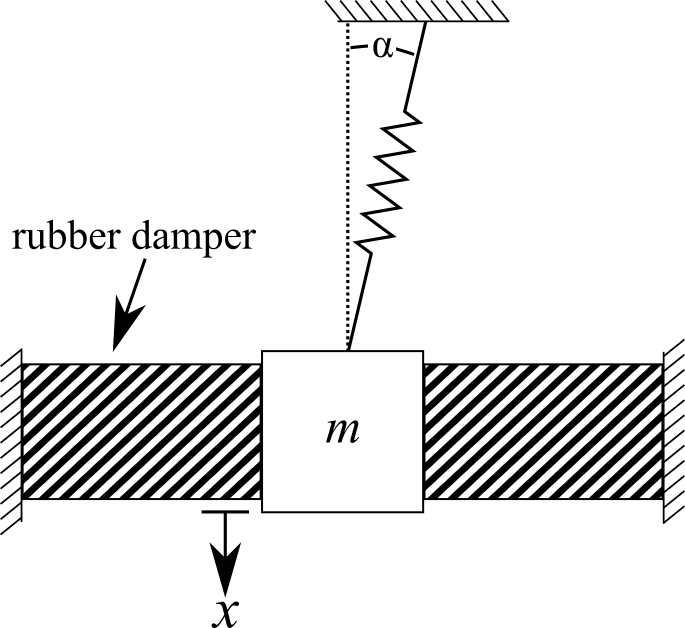
\includegraphics[]{../figures/rubber_mounted_mass_with_spring.png}
				\caption{Industrial device (mass) connected to a fixed point with a rubber damper and spring at an angle.}
				\label{fig:rubber_mounted_mass_with_spring}
			\end{figure}
	
			\noindent\textbf{Solution:} 
			
			\noindent First and foremost, we need to develop a mass-spring-dashpot representation of the system. This is presented in figure~\ref{fig:rubber_mounted_mass_with_spring_spring_dashpot_system} where the damping in the vertical direction provided by the rubber damper is modeled as a dashpot in the vertical direction. As we only want an estimate of the frequency, the assumption that the is small and as such $\alpha$ of the displaced state is equal $\alpha$ of the equilibrium state. 

			\begin{figure}[H]
				\centering
				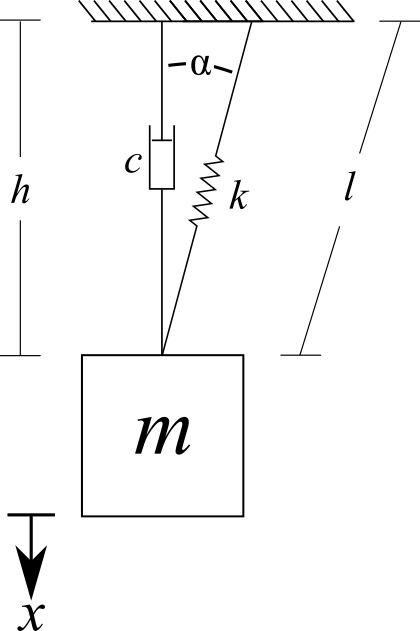
\includegraphics[]{../figures/rubber_mounted_mass_with_spring_spring_dashpot_system.png}
				\caption{Mass-spring-dashpot representation of the industrial system represented if figure \ref{fig:rubber_mounted_mass_with_spring}.}
				\label{fig:rubber_mounted_mass_with_spring_spring_dashpot_system}
			\end{figure}

			This leads to the FBD for the equilibrium  and displaced states:
			\begin{center}
				equilibrium position \hspace{4cm} displaced position ``x''
			\end{center}
			\begin{figure}[H]
				\centering
				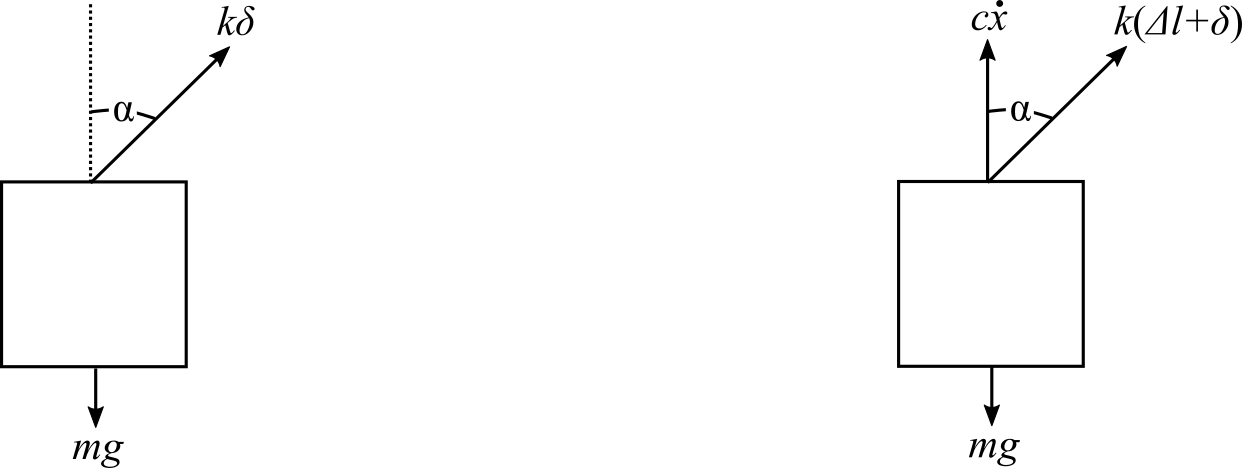
\includegraphics[]{../figures/rubber_mounted_mass_with_spring_FBD.png}
			\end{figure}
			The equation for the equilibrium state is:
			\begin{equation*}
				\downplus \sum F_x = mg -k\delta\text{cos}(\alpha) =0
			\end{equation*}
			and in the displaced state:
			\begin{equation*}
				\downplus \sum F_x = mg - c\dot{x}-k\text{cos}(\alpha)(\Delta l+\delta)
			\end{equation*}
			Applying Newton's second law and combining these equations yields:
			\begin{equation*}
				m\ddot{x} + c\dot{x} + k \Delta l \text{cos}(\alpha) =0
			\end{equation*}	
			Looking at the triangles formed by the dashpot and spring it can be shown that:
			\begin{equation*}
				 \cos(\alpha) = h/l = x/\Delta l  
			\end{equation*}			
			As we assumed the displacement is small and $\alpha$ remains unchanged. Therefore the prior equation becomes: 
			\begin{equation*}
				m\ddot{x} + c\dot{x} + k \Delta l \frac{x}{\Delta l} = 0
			\end{equation*}	
			This simplifies to the ``normal'' EOM for a 1-DOF system: 
			\begin{equation*}
				m\ddot{x} + c\dot{x} + k x  = 0
			\end{equation*}				
			Therefore, once the values for the system are measured the system's damped natural frequency in the vertical direction can be estimated as		
			\begin{equation*}
				\boxed{\omega_\text{d} = \omega_\text{n}\sqrt{1-\zeta^2}}
			\end{equation*}
		\end{example}	

	
		\begin{vibration_case_study}
			
		\textbf{Supplemental Damping in Automotive Damping}
		
		\noindent Epoxy-based damping is used in the automotive field to reduce vehicle noise and vibration harshness (NVH). This passive form of damping is essential for increasing comfort in modern light-wight vehicles. 
			
		\begin{figure}[H]
		\centering
		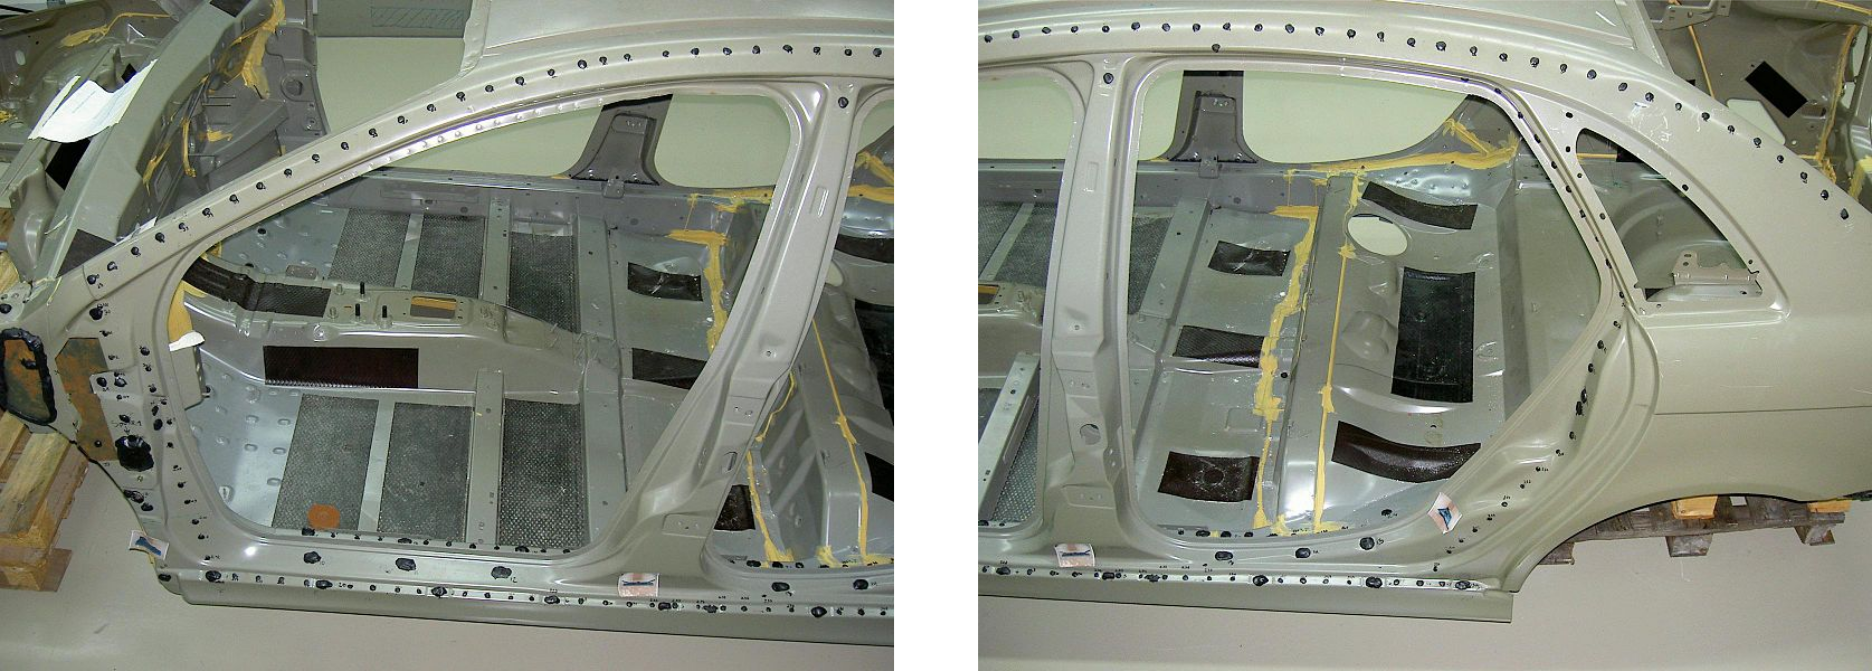
\includegraphics[width=6in]{../figures/automotive_epoxy_damping}
		\caption{Experimental modal analysis of an automotive (Jaguar) body in white, typically done to reduce vehicle noise and vibration harshness.\protect\footnotemark[1]}
			\footnotetext[1]{Cjp24, CC BY-SA 3.0 $<$https://creativecommons.org/licenses/by-sa/3.0$>$, via Wikimedia Commons.}
	\end{figure}		
		\end{vibration_case_study}
			
		\subsubsection{Modeling Overdamped Motion}
			
			In the case of overdamped systems, $1<\zeta$, the solutions for $\lambda$ are distinct real roots that are written as:
			\begin{equation}
				\lambda_{1} = -\zeta\omega_\text{n} - \omega_\text{n} \sqrt{\zeta^2-1}
			\end{equation} 			
			and:
			\begin{equation}
				\lambda_{2} = -\zeta\omega_\text{n} + \omega_\text{n} \sqrt{\zeta^2-1}
			\end{equation} 
			The solution for the EOM using the assumed solution then becomes:
			\begin{equation}
				x(t) = e^{-\zeta\omega_\text{n}t}(a_1e^{-\omega_\text{n} t \sqrt{\zeta^2-1}} + a_2e^{+\omega_\text{n} t \sqrt{\zeta^2-1}}) 
			\end{equation}
			This equation represents a non-oscillating response of the system. Again, $a_1$ and $a_2$ are solved for using known boundary conditions $x_0$ and $v_0$ such that:
			\begin{align}
				a_1 &= \frac{-v_0+\Big(-\zeta+\sqrt{\zeta^2-1}\Big)\omega_\text{n} x_0}{2\omega_\text{n}\sqrt{\zeta^2-1}} \\ 
				a_2 &= \frac{v_0+\Big(\zeta+\sqrt{\zeta^2-1}\Big)\omega_\text{n} x_0}{2\omega_\text{n}\sqrt{\zeta^2-1}}
			\end{align}				
			Typical responses for an overdamped system with various initial conditions are shown below in figure~\ref{fig:Over_damped_various_initial_conditions}.
			\begin{figure}[H]
				\centering
				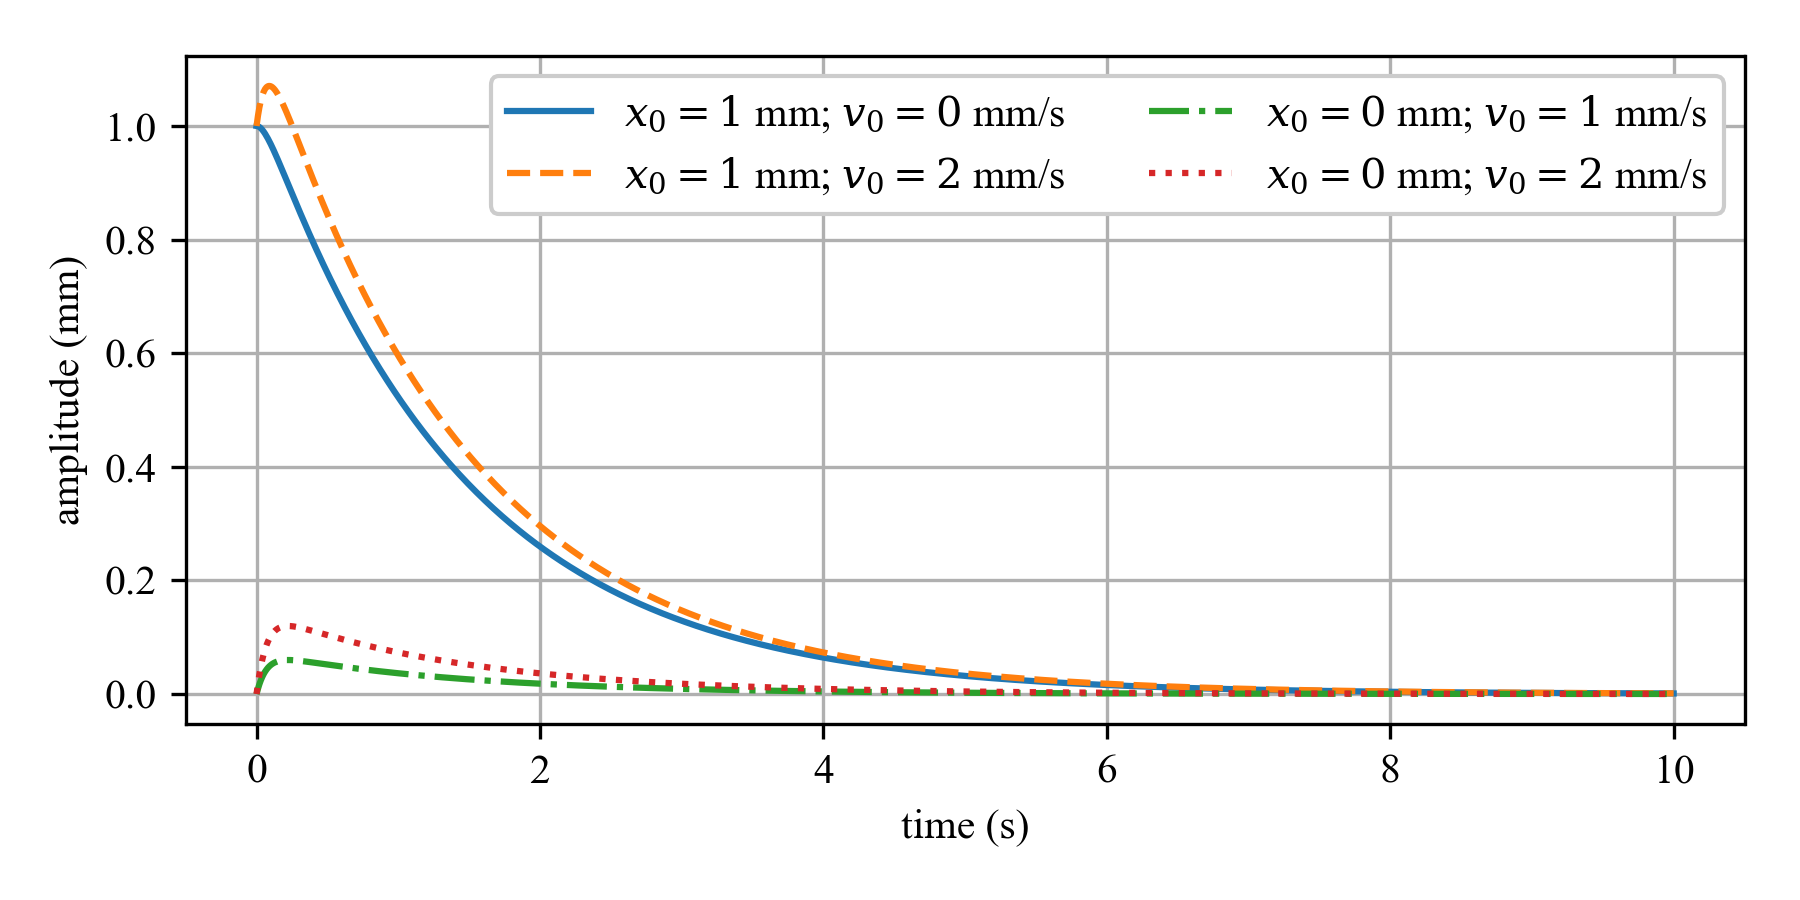
\includegraphics[]{../figures/Over_damped_various_initial_conditions.png}
				\caption{Four example responses for an overdamped 1-DOF system ($\zeta=2.371$) with various initial conditions.}
				\label{fig:Over_damped_various_initial_conditions}
			\end{figure}

		\subsubsection{Modeling Critically Damped Motion}			

			In the case of critically damped systems, $\zeta=1$, the solutions for $\lambda$ will be equal negative real numbers, therefore from before:
			\begin{equation}
				\lambda_{1,2} = -\zeta\omega_\text{n} \pm \omega_\text{n} \sqrt{\zeta^2-1}
			\end{equation}
			We get:
			\begin{equation}
				\lambda_{1} = \lambda_{2} = -\omega_\text{n}
			\end{equation} 			
			Because both solutions ($a_1$ and $a_2$) are the same, we multiply the second solution by $t$ so the solution for a critically damped system is in the same form as before. The solution for the EOM using the assumed solution then becomes:
			\begin{equation}
				x(t) = a_1e^{-\omega_\text{n}t} + a_2te^{-\omega_\text{n}t} 
			\end{equation} 
			This simplifies into:			
			\begin{equation}
				x(t) = (a_1+a_2t) e^{-\omega_\text{n}t} 
			\end{equation}
			This equation represents a non-oscillating response of the system. Again, $a_1$ and $a_2$ are solved for using known boundary conditions $x_0$ and $v_0$ such that:
			\begin{align}
				a_1 &= x_0 \\ 
				a_2 &= v_0+\omega_\text{n}x_0
			\end{align}				


		\subsubsection{Standard Form of the EOM}
			
			The EOM for a damped 1-DOF system is written in a ``standard form'' in which the effect of the damping ratio and natural frequencies are more obvious. To get to the standard form, the normal form of the EOM:
			\begin{equation}
				m\ddot{x} + c \dot{x} + kx = 0
			\end{equation}
			is divided by what the constant terms associated with the acceleration term. In this example, this is $m$. Dividing every term by $m$ yields: 
			\begin{equation}
				\ddot{x} + \frac{c}{m}\dot{x} + \frac{k}{m}x = 0
			\end{equation}		
			Numerical manipulations can be undertaken to get the coefficients of the velocity and displacement terms into coefficients that more clearly express the characteristics of the vibrating system:
			\begin{equation}
				\ddot{x} + 2\zeta\omega_\text{n}\dot{x} + \omega_\text{n}^2x = 0
			\end{equation}	

		\begin{example}

		\textbf{Vibration Modeling of Rocker Arm}

		\noindent An engine valve assembly is depicted in figure \ref{fig:engine_valve} where $J$ is the inertia caused by the right-hand side of the rocker arm. Derive an analytical solution for the natural frequency of the rocker arm. Use the assumptions sin($\theta$) = $\theta$ and cos($\theta$) = 1.
		
			\begin{figure}[H]
				\centering
				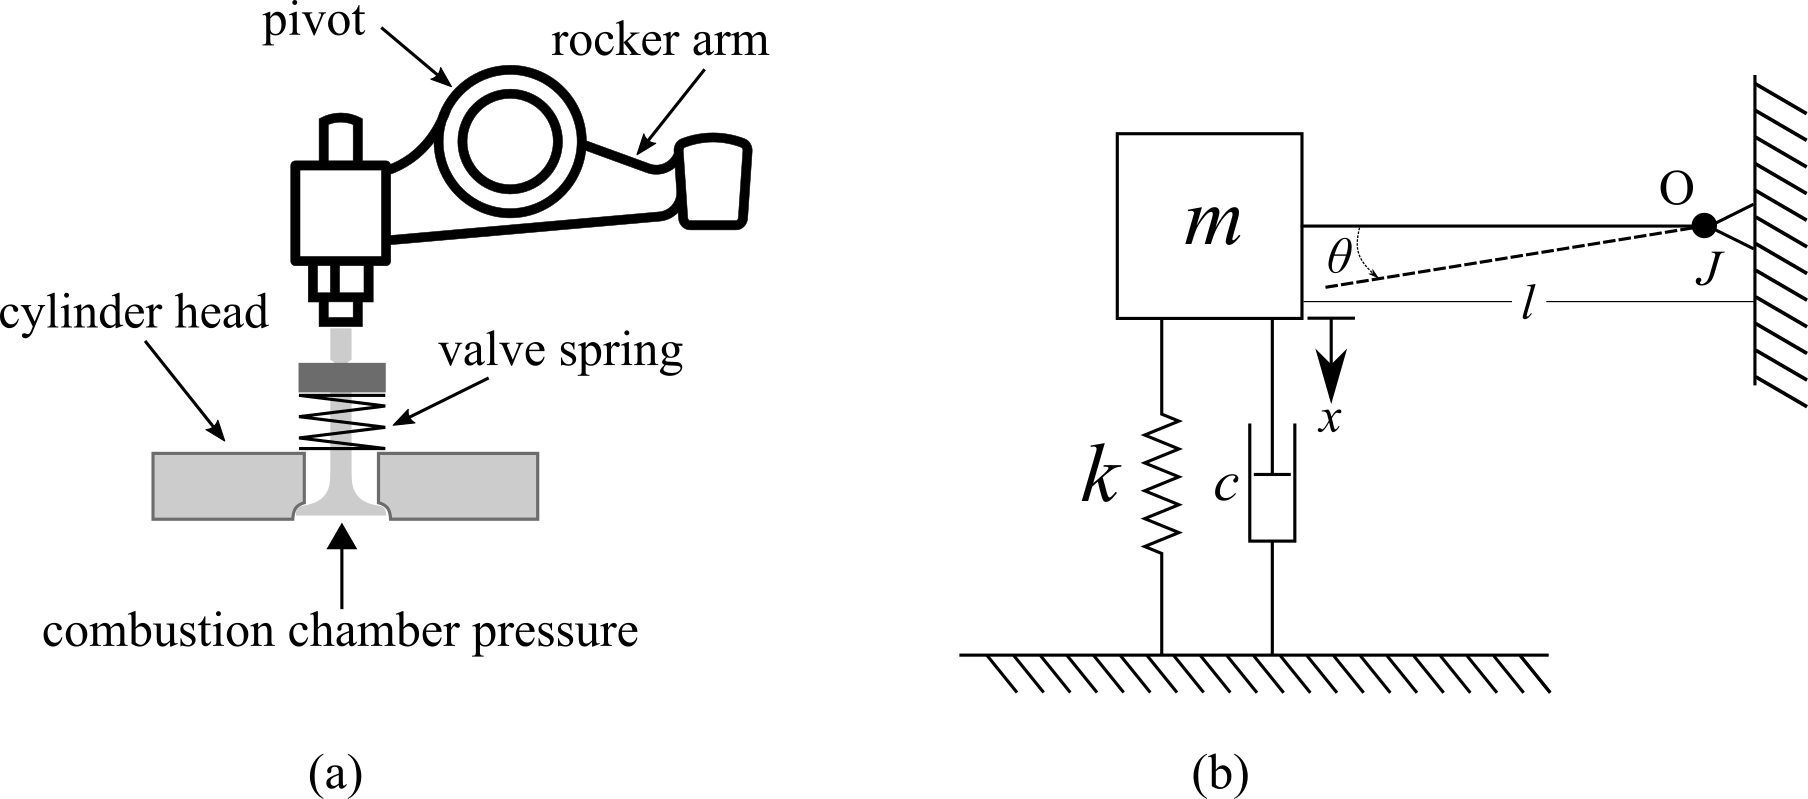
\includegraphics[]{../figures/engine_valve.png}
				\caption{Rocker arm assembly of an internal combustion engine showing: (a) a diagram of the system and; (b) the FBD of the system.}
				\label{fig:engine_valve}
			\end{figure}
			
		\noindent\textbf{Solution:} 
		
		\noindent Taking the sum of the moments about $O$ and considering the inertia caused by the right-hand side of the rocker arm, $J$, the FBDs can be written as: 
		\begin{center}
			equilibrium position \hspace{4cm} displaced position ``x''
		\end{center}
		\begin{figure}[H]
			\centering
			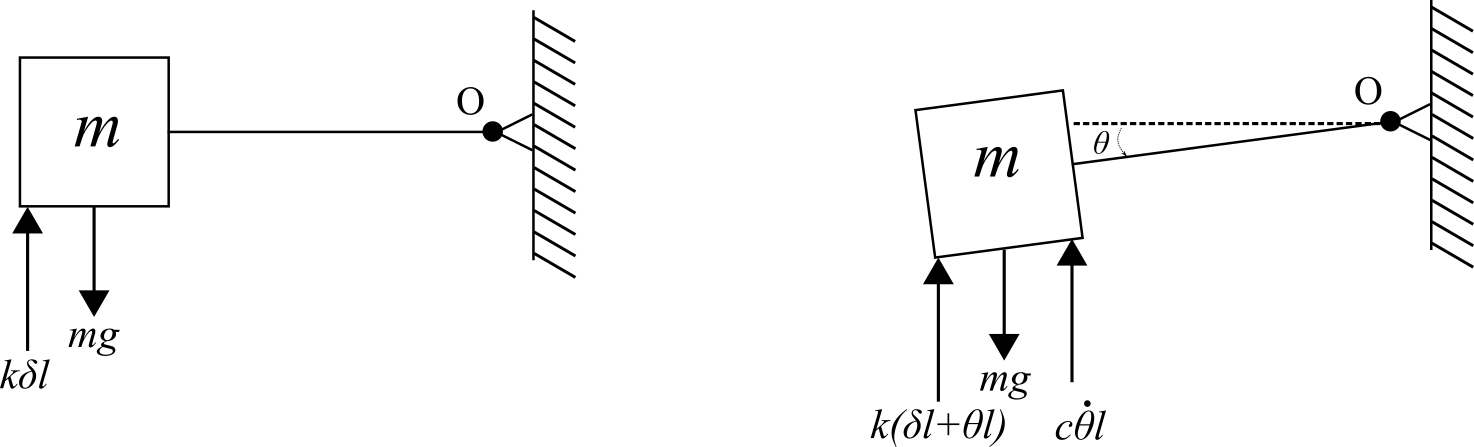
\includegraphics[]{../figures/engine_valve_FBD.png}
		\end{figure}
		The equation for the equilibrium state is:
		\begin{equation*}
			\curveplus \sum M_o = mgl -k l^2 \delta =0
		\end{equation*}
		and in the displaced state:
		\begin{equation*}
			\curveplus \sum M_o = mgl -k l^2 \delta -k l^2 \theta -c l^2\dot{\theta} =0
		\end{equation*}
		Applying Newton's second law and combining these equations yields:
		\begin{equation}
			(J+ml^2)\ddot{\theta} +cl^2\dot{\theta} + kl^2 \theta = 0
		\end{equation}	
		Therefore, the standard form of the EOM is:
		\begin{equation}
			\ddot{\theta} + \frac{cl^2}{J+ml^2}\dot{\theta} + \frac{kl^2 }{J+ml^2}\theta  = 0
		\end{equation}	
		Results in the following analytical solution for the natural frequency:
		\begin{equation}
			\omega_\text{n} = \sqrt{\frac{kl^2 }{J+ml^2}} \text{ rad/s}
		\end{equation}	
							
		\end{example}	


		\begin{vibration_case_study}
			
			\textbf{Vibration Induced Failure of Water Turbines}		

			\noindent On August 17\textsuperscript{th}, 2009 Turbine 2 of the hydroelectric power station of the Sayano-Shushenskaya Dam near Sayanogorsk in Russia failed catastrophically. The failure flooded the turbine hall and collapsed the ceiling. Killing 75 people, many of whom were in the turbine hall to celebrate the anniversary of the plant's general director.  Turbines of the type used at Sayano-Shushenskaya are designed to have high efficiency but a very narrow working band. When they operate outside the designed working band, they vibrate due to the pulsation of water flow and water strokes. These vibrations degrade the turbine over time. 
			
			Turbine 2 had experienced excessive vibrations for a long time, ever since its installation in 1979. Through the early 1980s several issues were fixed, along with substantial repairs in 2000 and 2005.  In July 2009 the turbine again exceeded the allowed vibration specification but stayed in operation. Over the years, the operating staff simply came to accept the higher level of vibration. The final government report stated that the accident was caused by turbine vibrations which led to fatigue damage in a turbine mount. 
			
			\begin{figure}[H]
				\centering
				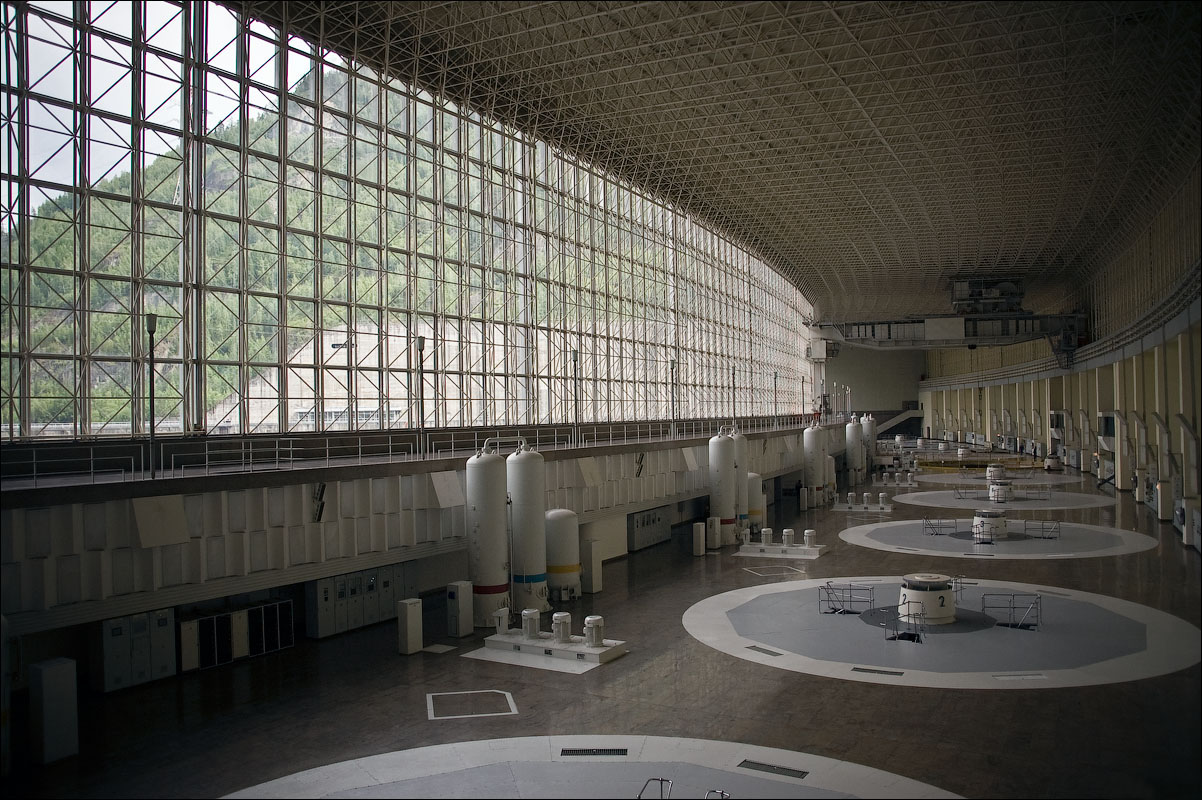
\includegraphics[width=4in]{../figures/Sayano-Shushenskaya_HPS_-_generator_hall}
				\caption{Sayano Shushenskaya's turbine hall before the accident where turbine 2 (the turbine that failed) is in the foreground of the image. \protect\footnotemark[1]}
			\end{figure}

			\begin{figure}[H]
				\centering
				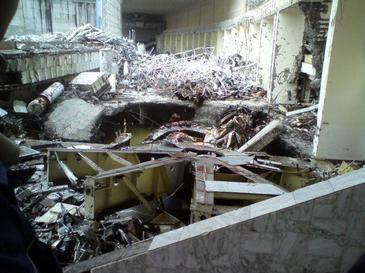
\includegraphics[width=4in]{../figures/Sayano-Shushenskaya_HPS_-_generator_hall_post-accident}
				\caption{Sayano Shushenskaya's turbine hall after the accident. \protect\footnotemark[2] \bl{} }
			\end{figure}
			
%			\begin{otherlanguage*}{russian}
%			????? ?? ??????? ?????
%			\end{otherlanguage*}

			\footnotetext[1]{4044415 \foreignlanguage{russian}{Russian: Andrey Korzun} English:  Andrey Korzun, CC BY-SA 3.0 $<$https://creativecommons.org/licenses/by-sa/3.0$>$, via Wikimedia Commons}
			\footnotetext[2]{The original source of this photograph is believed to be Jaffaa, a user of forums.drom.ru, who uploaded it on August 17, 2009, a few hours after the accident. This image is a faithful digitization of a unique historic image, and the copyright for it is most likely held by the person who created the image or the agency employing the person. It is believed that the use of this image may qualify as fair use under the copyright law of the United States.}

		\end{vibration_case_study}

 
	
%	4044415 ???????:  ?????? ?????? English:  Andrey Korzun, CC BY-SA 3.0 <https://creativecommons.org/licenses/by-sa/3.0>, via Wikimedia Commons
	
		\subsection{Logarithmic Decrement}
			
			For a vibrating system, the mass ($m$) and stiffness ($k$) can be measured using scales and static deflection tests. However, the damping coefficient ($c$) is a more difficult quantity to determine. From $k$ and $m$ we can compute the natural frequency ($\omega_\text{n}$) and the critical damping coefficient ($c_\text{cr}$). Therefore, knowing that the critical damping ratio ($\zeta$) is defined as:
			\begin{equation}
				\zeta = \frac{c}{c_{\text{cr}}} = \frac{c}{2\sqrt{km}} = \frac{c}{2m\omega_\text{n}}
			\end{equation}				
			if we calculate $\zeta$, we can obtain $c$ for the system of interest. This is made possible because $c_\text{cr}$ can be calculated from $k$ and $m$. Observing the temporal response for the underdamped system, 
			\begin{figure}[H]
				\centering
				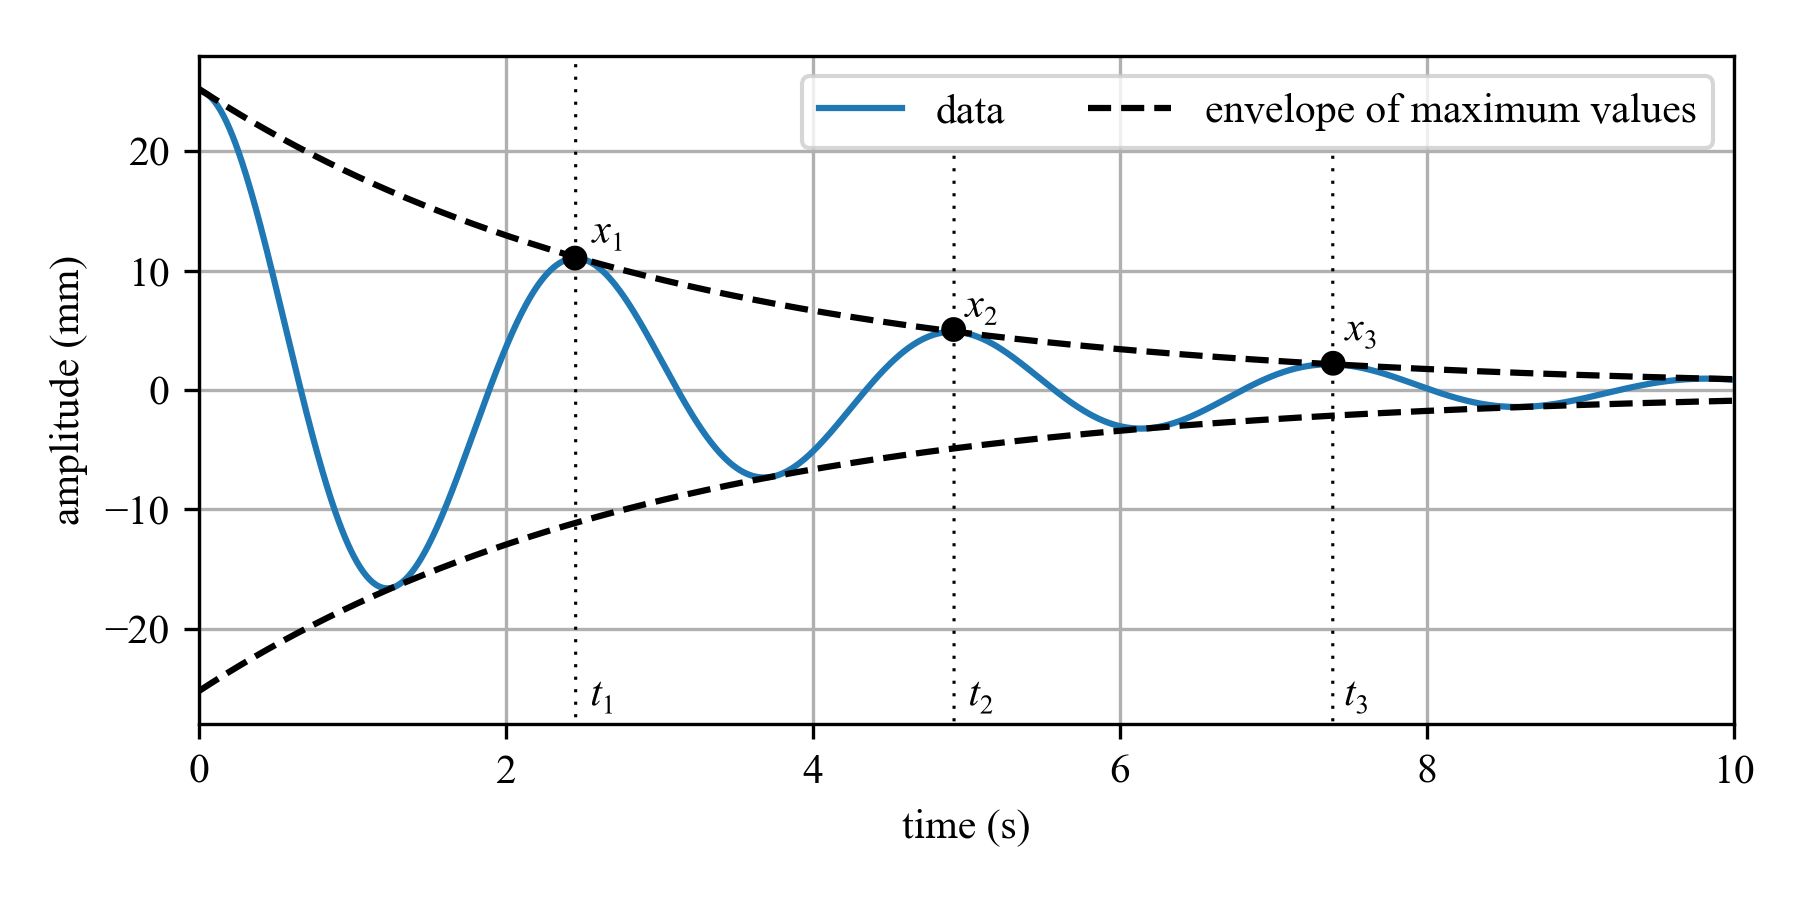
\includegraphics[]{../figures/Logarithmic_decrement.png}
				\caption{Measuring the peak displacement points in an experimental system with decay caused by damping.}
			\end{figure}
			
			\noindent we mark three points of maximum amplitude, $x_1$, $x_2$, and $x_3$ that happen at $t_1$, $t_2$, and $t_3$, respectively. Considering displacement values for the first two points $x_1$ and $x_2$, separated by a complete period ($T$).  Knowing that one cycle is $2 \pi$, the time period for this complete cycle is given by:
			\begin{equation}
				t_2-t_1 = \frac{2\pi}{\omega_\text{d}} = \frac{2\pi}{\omega_\text{n}\sqrt{1-\zeta^2}}
			\end{equation}				
			where $\omega_\text{d}$ is the damped natural frequency. This is the time period ($T$) of damped oscillations. If we derive an equation for the values of the peaks, also called the envelope of maximum values, we get: 
			\begin{equation}
				x_{\text{peaks}} = Ae^{-\zeta\omega_\text{n}t} 
			\end{equation} 		
			Knowing that the system is underdamped, $A$ can be solved for using the initial conditions $x_0$ and $v_0$, therefore: 
			\begin{equation}
				A = \frac{\sqrt{(v_0+\zeta\omega_\text{n}x_0)^2 + (x_0\omega_\text{d})^2}}{\omega_\text{d}}
			\end{equation} 	
			In terms of $t_1$ and $t_2$, we can express the displacement at these times as:
			\begin{equation}
				x_{\text{1}} = A e^{-\zeta \omega_\text{n} t_1}
			\end{equation}				
			and 
			\begin{equation}
				x_{\text{2}} = A e^{-\zeta \omega_\text{n} t_2}
			\end{equation}		
			therefore:
			\begin{equation}
				\frac{x_{\text{1}}}{x_{\text{2}}} = \frac{e^{-\zeta \omega_\text{n} t_1}}{e^{-\zeta \omega_\text{n} t_2}} = e^{\zeta \omega_\text{n}(t_2-t_1)}
			\end{equation}		
			However, from before we know that $t_2-t_1 = \frac{2\pi}{\omega_\text{d}} = \frac{2\pi}{\omega_\text{n}\sqrt{1-\zeta^2}}$. Therefore, we can express this last equation as:
			\begin{equation}
				\frac{x_{\text{1}}}{x_{\text{2}}} =e^{\Big(\frac{2 \pi \zeta}{\sqrt{1-\zeta^2}}\Big)}
			\end{equation}			
			Next, we take the natural log of both sides to get the logarithmic decrement, denoted by $\delta$:
			\begin{equation}
				\delta = \text{ln}\bigg(\frac{x_{\text{1}}}{x_{\text{2}}}\bigg) = \text{ln}\bigg(\frac{x(t_{\text{1}})}{x(t_{\text{1}}+T)}\bigg) = \frac{2 \pi \zeta}{\sqrt{1-\zeta^2}}
			\end{equation}				
			This shows us that the ratio of any two successive amplitudes for an underdamped system, vibrating freely, is constant and is a function of the damping only. Sometimes, in experiments, it is more convenient/accurate to measure the amplitudes after say ``$n$'' peaks rather than two successive peaks (because if the damping is very small, the difference between the successive
			peaks may not be significant). The logarithmic decrement can then be given by the equation
			\begin{equation}
				\delta = \frac{1}{n}\text{ln}\bigg(\frac{x_{\text{1}}}{x_{\text{n+1}}}\bigg) =   \frac{1}{n}\text{ln}\bigg(\frac{x(t_{\text{1}})}{x(t_{\text{1}}+nT)}\bigg) = \frac{2 \pi \zeta}{\sqrt{1-\zeta^2}}
			\end{equation}				
			Once we use the experimental data to obtain $\delta$, and knowing that:
			\begin{equation}
				\delta = \frac{2 \pi \zeta}{\sqrt{1-\zeta^2}}
			\end{equation}	
			we can calculate the value of $\zeta$:
			\begin{equation}
				\zeta = \frac{\delta}{\sqrt{4\pi^2+\delta^2}}
			\end{equation}
			Therefore, having $\zeta$ we can solve for the coefficient of damping, $c$, as: 
			\begin{equation}
				c = \zeta 2\sqrt{km}
			\end{equation}					

			\begin{example}
			\textbf{Experimentally Measuring System Damping}
			
			\noindent Calculate the damping coefficient for the system with the measured amplitude as expressed below given that $m$ = 3 kg and $k$ = 43 N/m. Use $t_1$ = 1 sec, and $t_{n+1} =t_4=6$ sec. Use the peaks as marked in figure~\ref{fig:Logarithmic_decrement_with_noise}.

			\begin{figure}[H]
				\centering
				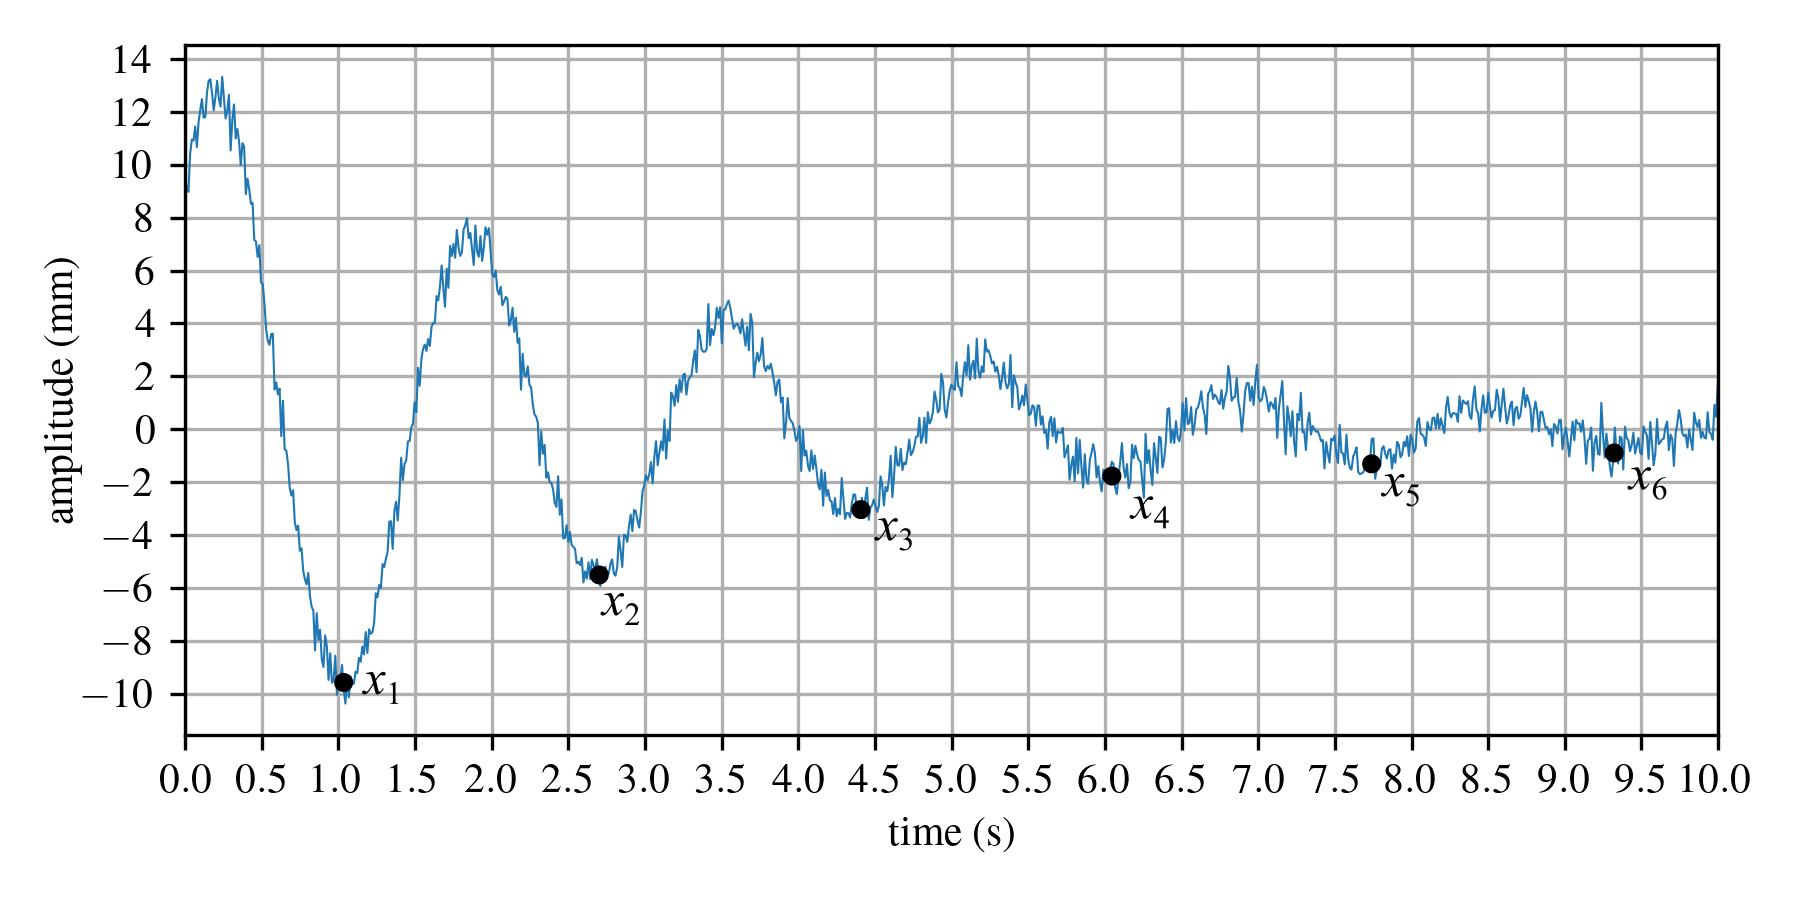
\includegraphics[]{../figures/Logarithmic_decrement_with_noise.png}
				\caption{Response from an experimental system with noise.}
				\label{fig:Logarithmic_decrement_with_noise}
			\end{figure}
			
			\noindent\textbf{Solution:} 
						
			First, from the plot we can determine that $x_1=-9.5$ mm and $x_4=-1.8$ mm where $n=3$. Thereafter, we can solve for $\delta$:  
			\begin{equation}
				\delta = \frac{1}{3}\text{ln}\bigg(\frac{x_{\text{1}}}{x_{\text{4}}}\bigg) = \frac{1}{3}\text{ln}\bigg(\frac{-9.5}{-1.8}\bigg) = 0.554
			\end{equation}						
			Next, we can calculate $\zeta$, as: 
			\begin{equation}
				\zeta = \frac{\delta}{\sqrt{4\pi^2+\delta^2}} = \frac{0.554}{\sqrt{4\pi^2+0.554^2}} = 0.0879
			\end{equation}
			And lastly:			
			\begin{equation}
				c = \zeta 2\sqrt{km} = 0.0879 \cdot 2\sqrt{43 \cdot 3} = 2.0 \text{ kg/s}
			\end{equation}	

			\end{example}

	
			\begin{example}
			
			\textbf{Calculating Damping Coefficient}
			
			\noindent The free-response of a 1000-kg automobile with stiffness of $k$ = 400,000 N/m is observed to be underdamped. Modeling the automobile as a single-degree-of-freedom oscillation in the vertical direction, as annotated in figure \ref{fig:vehicle_wheel_undamped}, determine the damping coefficient if the displacement at $t_1$ is measured to be 2 cm and 0.22 cm at $t_2$.

			\noindent\textbf{Solution:} 
					
			\noindent Knowing $x_1$ = 2 cm and $x_2$ = 0.22 cm and $t_2 = T + t_1$, therefore:
			\begin{equation}
				\delta = \text{ln}\frac{x_1}{x_2} = \text{ln}\frac{2}{0.22} = 2.207
			\end{equation}			
			and:
			\begin{equation}
				\zeta = \bigg(\frac{\delta}{\sqrt{4\pi^2+\delta^2}}\bigg) = \bigg(\frac{2.207}{\sqrt{4\pi^2+2.207^2}}\bigg) = 0.331
			\end{equation}
			therefore, we can obtain the damping coefficient as
			\begin{equation}
				c = 2\zeta\sqrt{km}=2(0.331)\sqrt{400,000 \cdot 1,000} = 13,256 \hspace{1ex} 
				\text{kg/s} 
			\end{equation}	

\end{example}
		
						
			
			


\end{document}